\section{Simulations}\label[sec]{results}
Simulations are done in four different mission spaces with properties summed up in Table \ref{tab:worlds}.
\begin{center}
  \captionof{table}{Mission space properties\label{tab:worlds}}
  \begin{tabular}{l|l|l}
    Name & Size & Obstacles\\
    \hline
    Tinyworld & 1.5-by-1.5 square & None\\
    Tinyworld2 & 1.5-by-1.5 square & Central 0.5-by-0.5 square\\
    Rectworld & 10-by-10 square & None\\
    Complexworld & Pentagon & Horizontal wall, vertical wall and hexagon
  \end{tabular}
\end{center}
For all mission spaces simulations are performed where the dispersion term is neglected ($k_{1} = 0$), i.e.
$H(\mathbf{X}_{\mathcal{B}_{a}\cup\{a\}}) = L(\mathbf{X}_{\mathcal{B}_{a}\cup\{a\}})$, and where the dispersion term
is present ($k_{1} = 1$).
\clearpage
\subsection{Tinyworld}\label[secc]{tinyworld}
The Tinyworld is constructed so that for three or more agents, the entire feasible space is covered regardless of the position of the agents.

\Cref{fig:3_agnt_tw_k_1_0_distr} shows the initial and final configuration of 3 agents when spawned in the Tinyworld environment, 
and no active dispersion is used ($k_{1} = 0$).
\Cref{fig:3_agnt_tw_evolution} shows the covered area and step length per agent versus iteration count.

Results of optimizing agent positions with active dispersion ($k_{1} = 1$, $k_{2} = 1$) are shown in \Crefrange{fig:3_agnt_tw_k_1_1_k_2_1_distr}{fig:3_agnt_tw_evolution_active}.

\begin{figure}[H]
  \centering
  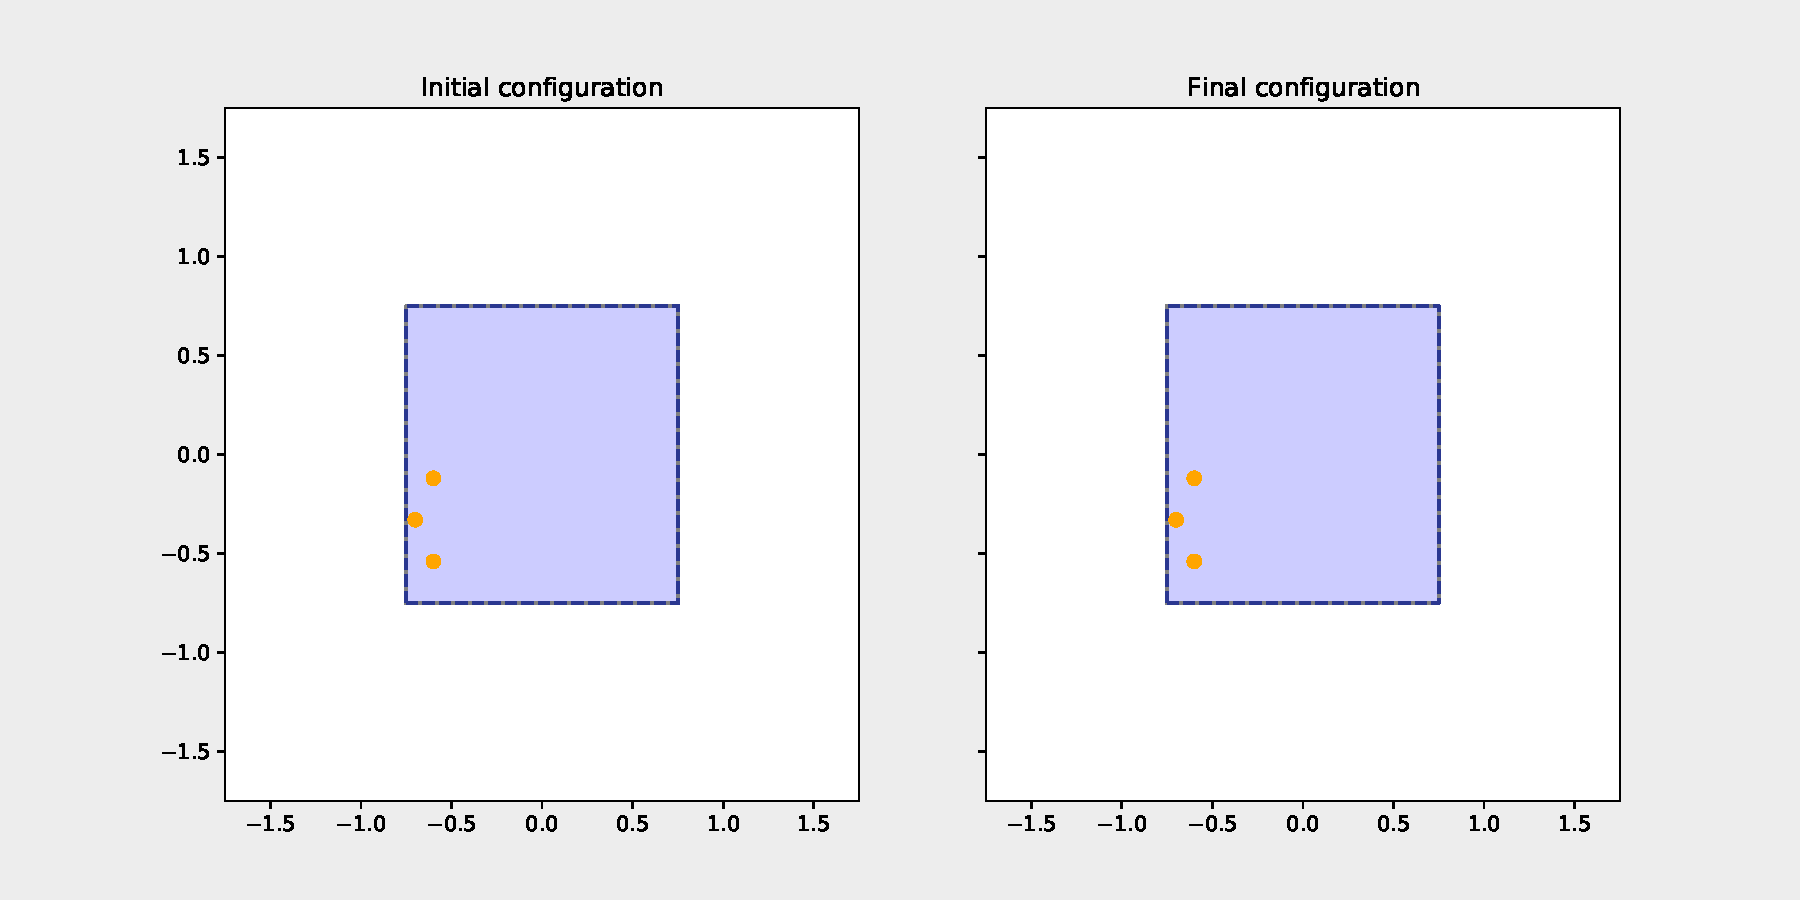
\includegraphics[width=\textwidth]{figs/tinyworld_3_agnt_k_1_0_k_2_1_distr.pdf}
  \caption{Initial and final configuration of 3 agents in the Tinyworld environment with $k_{1} = 0$ (no active dispersion).}
  \label{fig:3_agnt_tw_k_1_0_distr}
\end{figure}

\begin{figure}[H]
  \centering
  \begin{subfigure}[t]{0.5\textwidth}
    \centering
    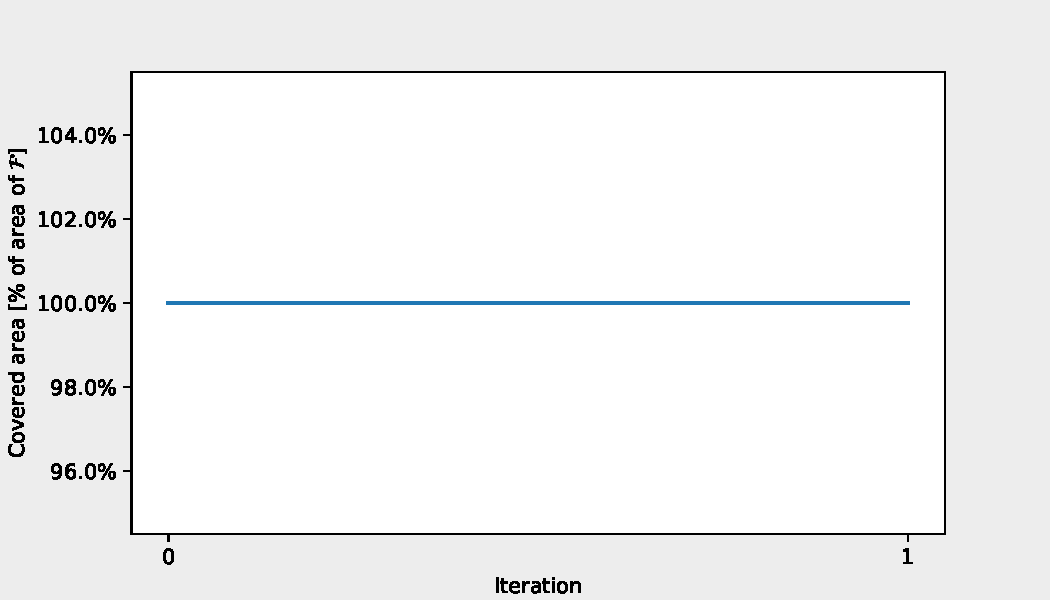
\includegraphics[width=\textwidth]{figs/tinyworld_3_agnt_k_1_0_k_2_1_area_traj.pdf}
    \caption{Coverage evolution for 3 agents in the Tinyworld environment with $k_{1} = 0$ (no active dispersion).}
    \label{fig:3_agnt_tw_k_1_0_a_traj}
  \end{subfigure}%
  ~ 
  \begin{subfigure}[t]{0.5\textwidth}
    \centering
    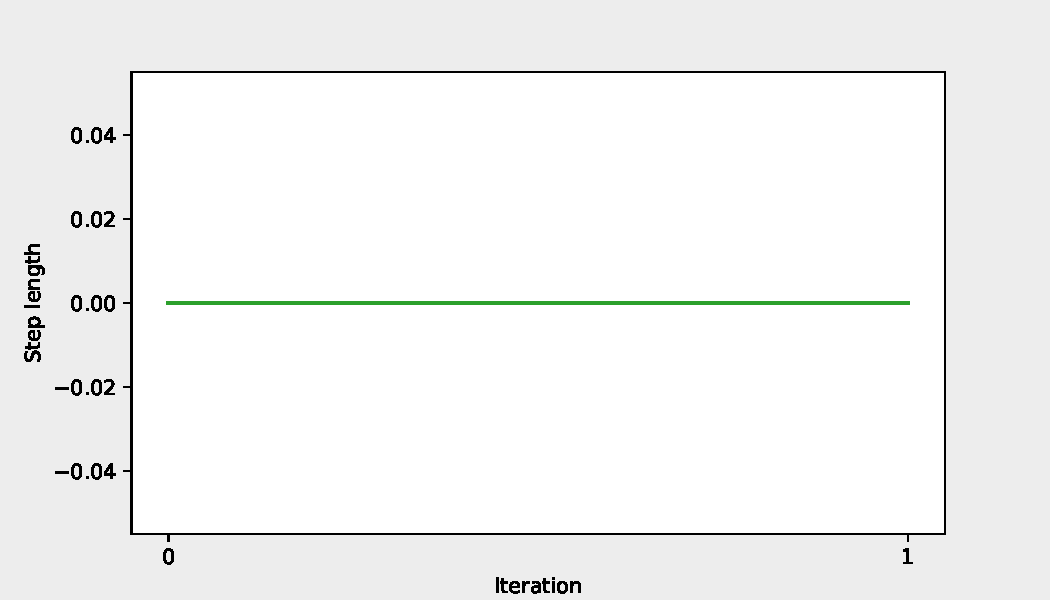
\includegraphics[width=\textwidth]{figs/tinyworld_3_agnt_k_1_0_k_2_1_step_traj.pdf}
    \caption{Step length evolution for 3 agents in the Tinyworld environment with $k_{1} = 0$ (no active dispersion).}
    \label{fig:3_agnt_tw_k_1_0_s_traj}
  \end{subfigure}
  \caption{Coverage percentage and step length evolution for 3 agents in the Tinyworld environment when no active dispersion is used.}
  \label{fig:3_agnt_tw_evolution}
\end{figure}

\begin{figure}[H]
  \centering
  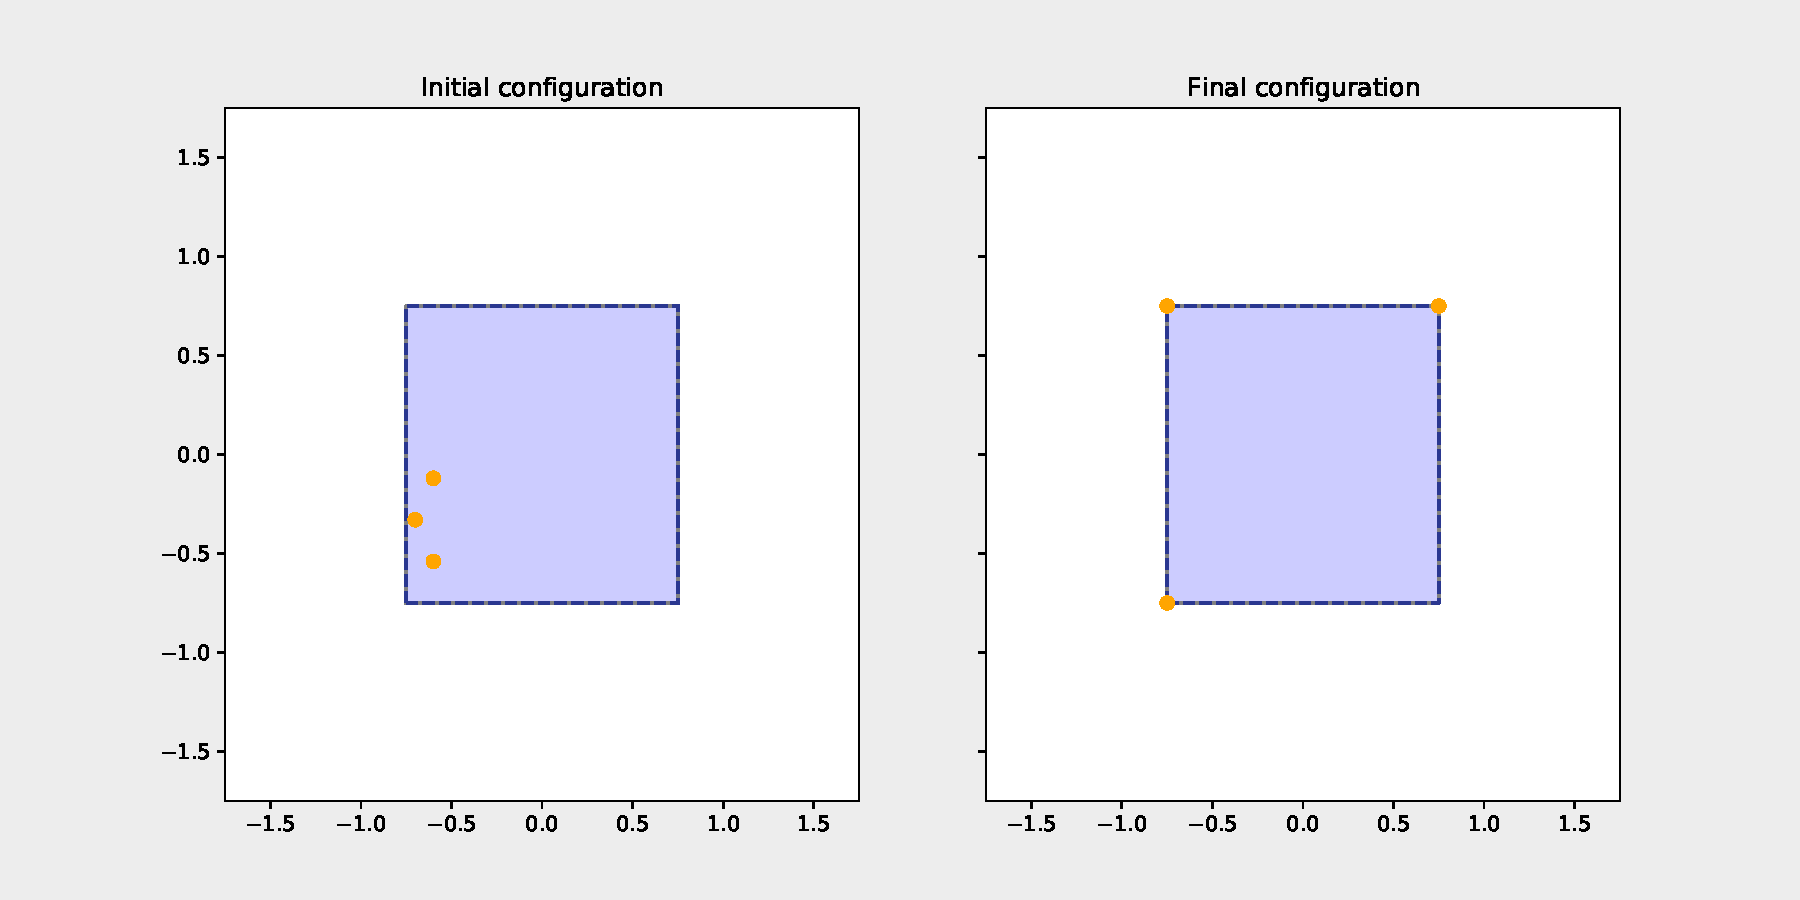
\includegraphics[width=\textwidth]{figs/tinyworld_3_agnt_k_1_1_k_2_1_distr.pdf}
  \caption{Initial and final configuration of 3 agents in the Tinyworld environment with $k_{1} = k_{2} = 1$ (active dispersion).}
  \label{fig:3_agnt_tw_k_1_1_k_2_1_distr}
\end{figure}

\begin{figure}[H]
  \centering
  \begin{subfigure}[t]{0.5\textwidth}
    \centering
    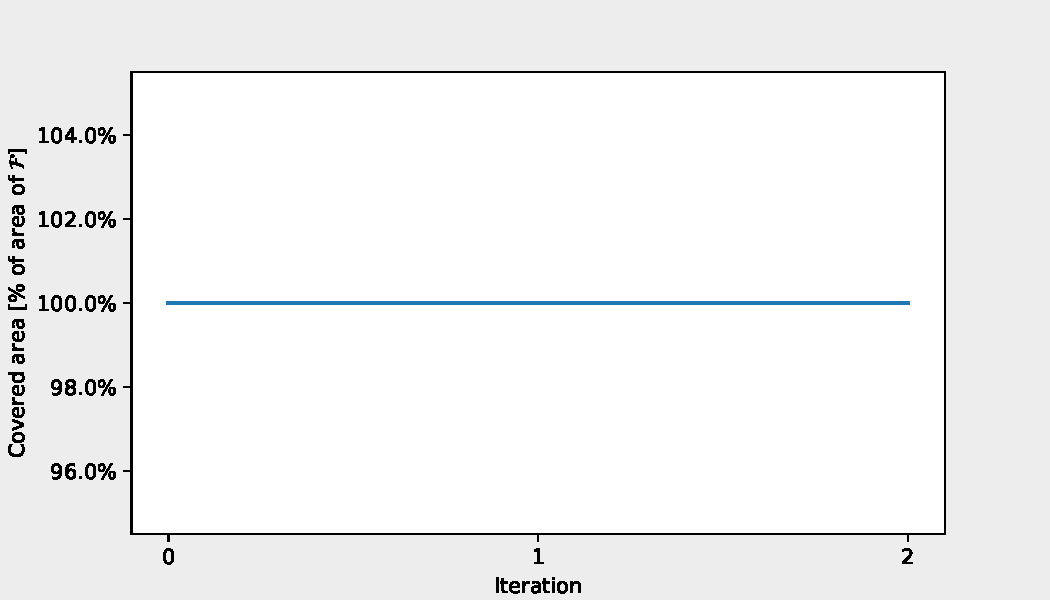
\includegraphics[width=\textwidth]{figs/tinyworld_3_agnt_k_1_1_k_2_1_area_traj.pdf}
    \caption{Coverage evolution for 3 agents in the Tinyworld environment with $k_{1} = k_{2} = 1$ (active dispersion).}
    \label{fig:3_agnt_tw_k_1_k_2_1_a_traj}
  \end{subfigure}%
  ~ 
  \begin{subfigure}[t]{0.5\textwidth}
    \centering
    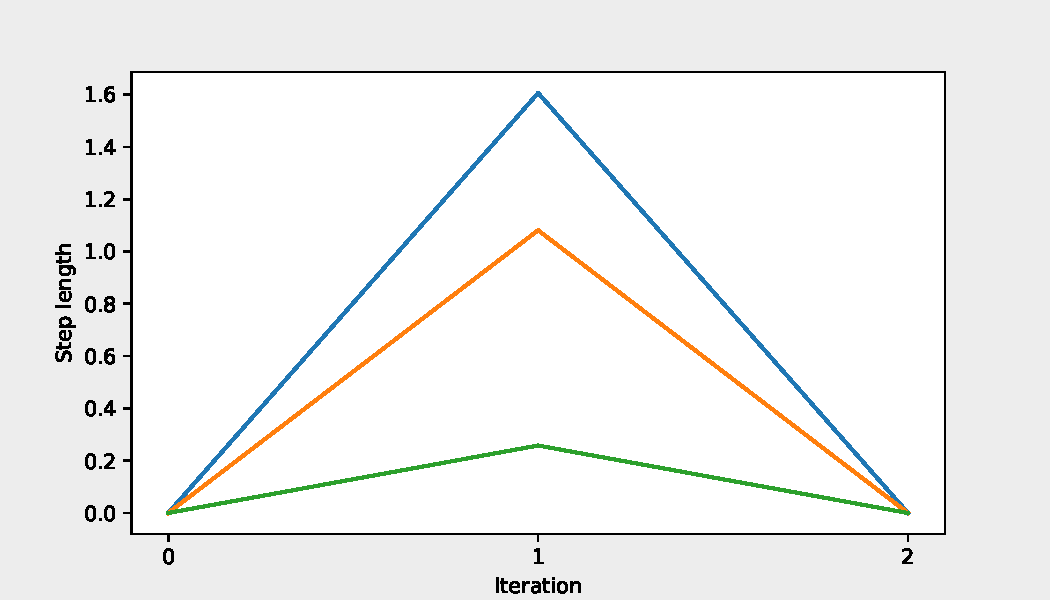
\includegraphics[width=\textwidth]{figs/tinyworld_3_agnt_k_1_1_k_2_1_step_traj.pdf}
    \caption{Step length evolution for 3 agents in the Tinyworld environment with $k_{1} = k_{2} = 1$ (active dispersion).}
    \label{fig:3_agnt_tw_k_1_k_2_1_s_traj}
  \end{subfigure}
  \caption{Coverage percentage and step length evolution for 3 agents in the Tinyworld environment when active dispersion is used.}
  \label{fig:3_agnt_tw_evolution_active}
\end{figure}
\clearpage
\subsection{Tinyworld2}\label[secc]{tinyworld2}
The Tinyworld2 environment is constructed to study how obstacles affect the configuration generated by Algorithm \ref{alg:alg1}.

The results of a simulation for 3 agents without active dispersion ($k_{1} = 0$) is shown in \Crefrange{fig:3_agnt_tw2_k_1_0_distr}{fig:3_agnt_tw2_evolution}.
\Crefrange{fig:6_agnt_tw2_k_1_0_distr}{fig:6_agnt_tw2_evolution} show the results of a simulation of 6 agents without active dispersion.

The results generated by Algorithm \ref{alg:alg1} when applying active dispersion ($k_{1} = 1$, $k_{1} = 2$) and running simulations for 3 and 6 agents 
are shown in \Crefrange{fig:3_agnt_tw2_k_1_1_k_2_1_distr}{fig:3_agnt_tw2_evolution_active} and \Crefrange{fig:6_agnt_tw2_k_1_1_k_2_1_distr}{fig:6_agnt_tw2_evolution_active} respectively.
\begin{figure}[H]
  \centering
  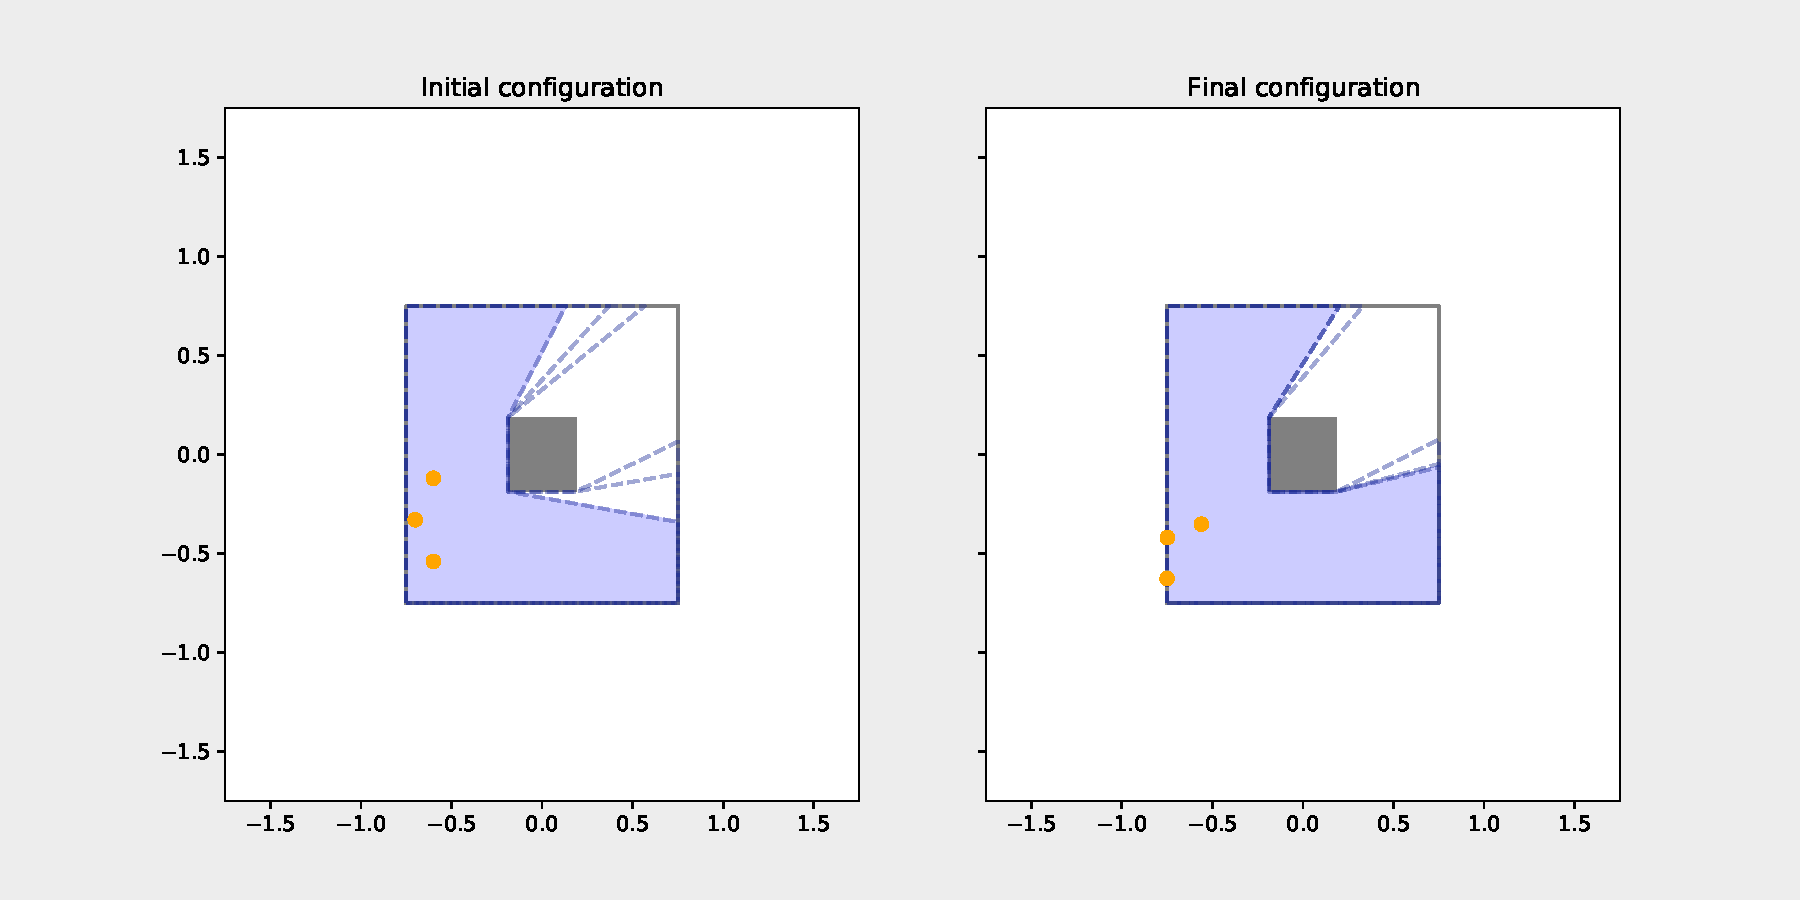
\includegraphics[width=\textwidth]{figs/tinyworld2_3_agnt_k_1_0_k_2_1_distr.pdf}
  \caption{Inital and final configuration of 3 agents in the Tinyworld2 environment with $k_{1} = 0$ (no active dispersion).}
  \label{fig:3_agnt_tw2_k_1_0_distr}
\end{figure}
\begin{figure}[H]
  \centering
  \begin{subfigure}[t]{0.5\textwidth}
    \centering
    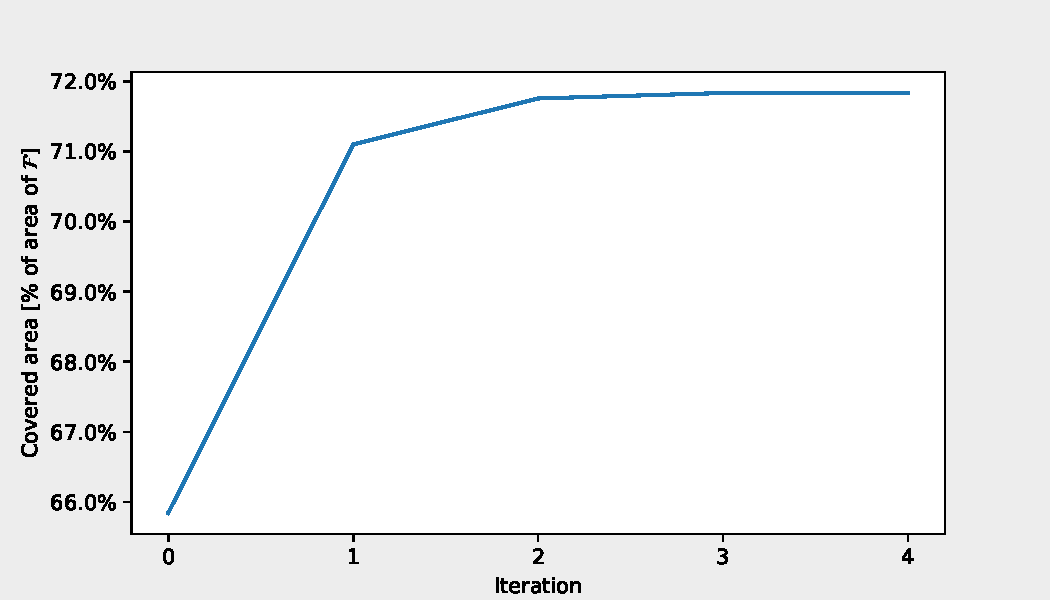
\includegraphics[width=\textwidth]{figs/tinyworld2_3_agnt_k_1_0_k_2_1_area_traj.pdf}
    \caption{Coverage evolution for 3 agents in the Tinyworld2 environment with $k_{1} = 0$ (no active dispersion).}
    \label{fig:3_agnt_tw2_k_1_0_a_traj}
  \end{subfigure}%
  ~ 
  \begin{subfigure}[t]{0.5\textwidth}
    \centering
    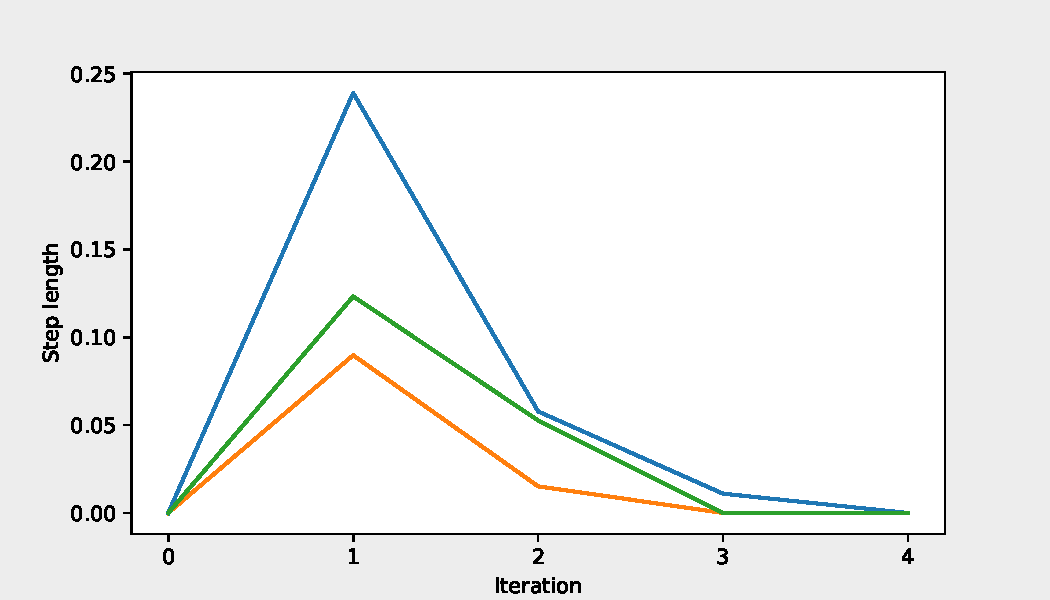
\includegraphics[width=\textwidth]{figs/tinyworld2_3_agnt_k_1_0_k_2_1_step_traj.pdf}
    \caption{Step length evolution for 3 agents in the Tinyworld2 environment with $k_{1} = 0$ (no active dispersion).}
    \label{fig:3_agnt_tw2_k_1_0_s_traj}
  \end{subfigure}
  \caption{Coverage percentage and step length evolution for 3 agents in the Tinyworld2 environment when no active dispersion is used.}
  \label{fig:3_agnt_tw2_evolution}
\end{figure}


\begin{figure}[H]
  \centering
  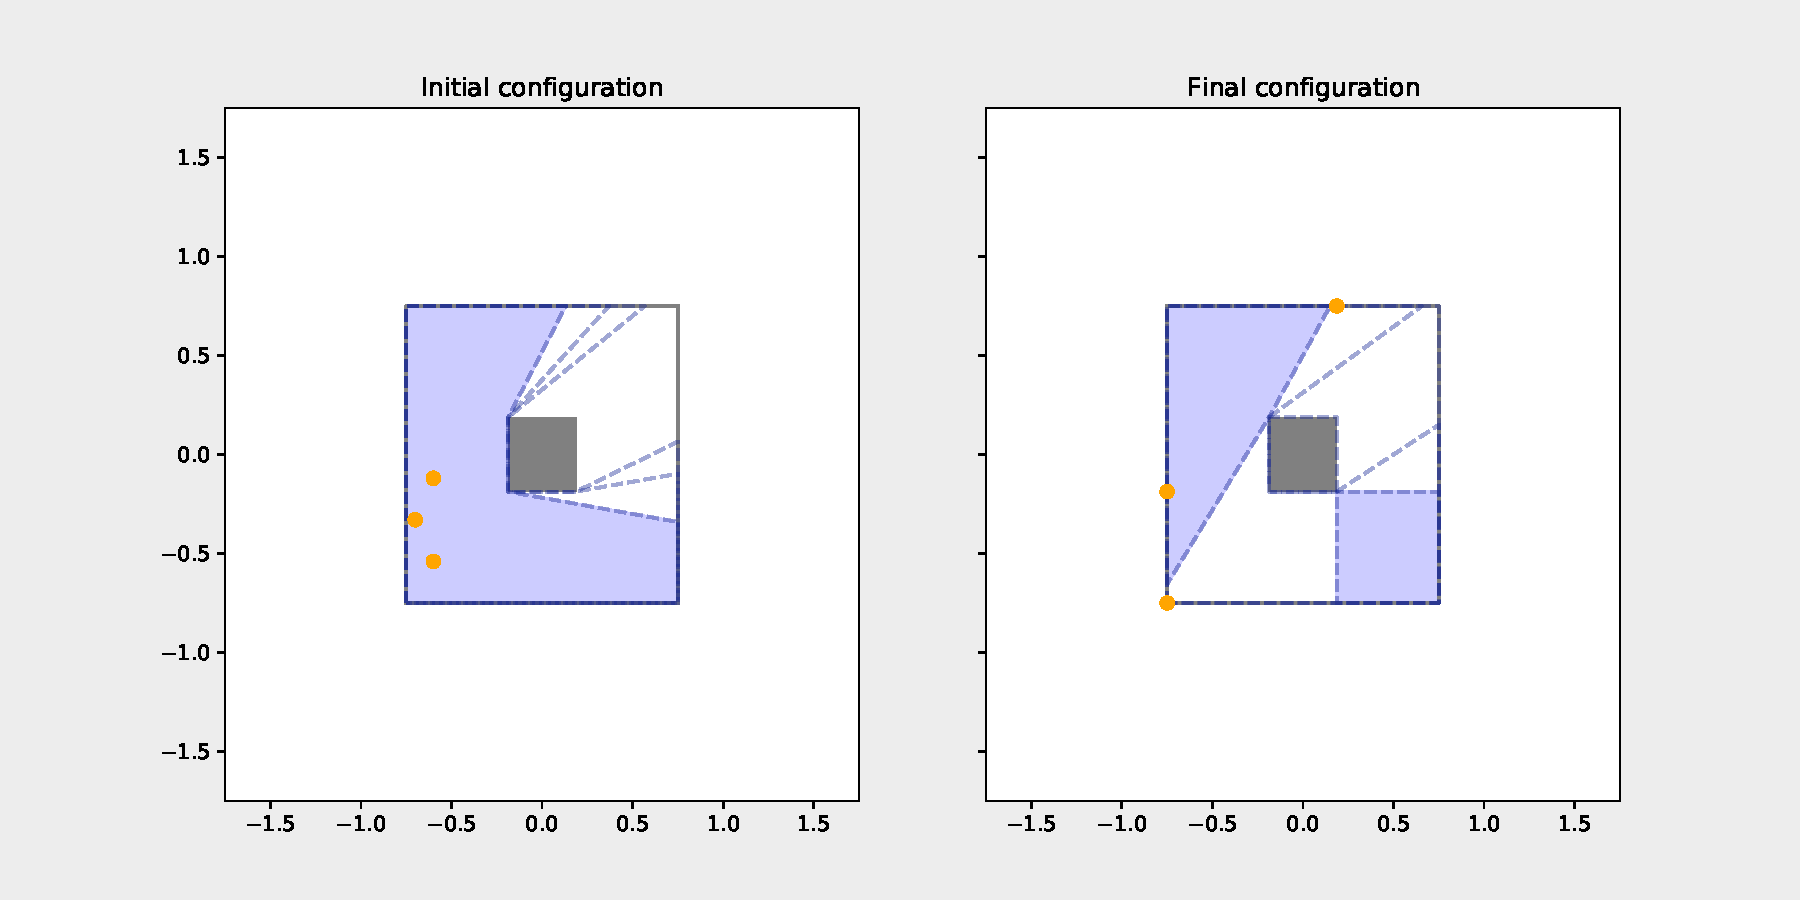
\includegraphics[width=\textwidth]{figs/tinyworld2_3_agnt_k_1_1_k_2_1_distr.pdf}
  \caption{Inital and final configuration of 3 agents in the Tinyworld2 environment with $k_{1} = k_{2} = 1$ (active dispersion).}
  \label{fig:3_agnt_tw2_k_1_1_k_2_1_distr}
\end{figure}
\begin{figure}[H]
  \centering
  \begin{subfigure}[t]{0.5\textwidth}
    \centering
    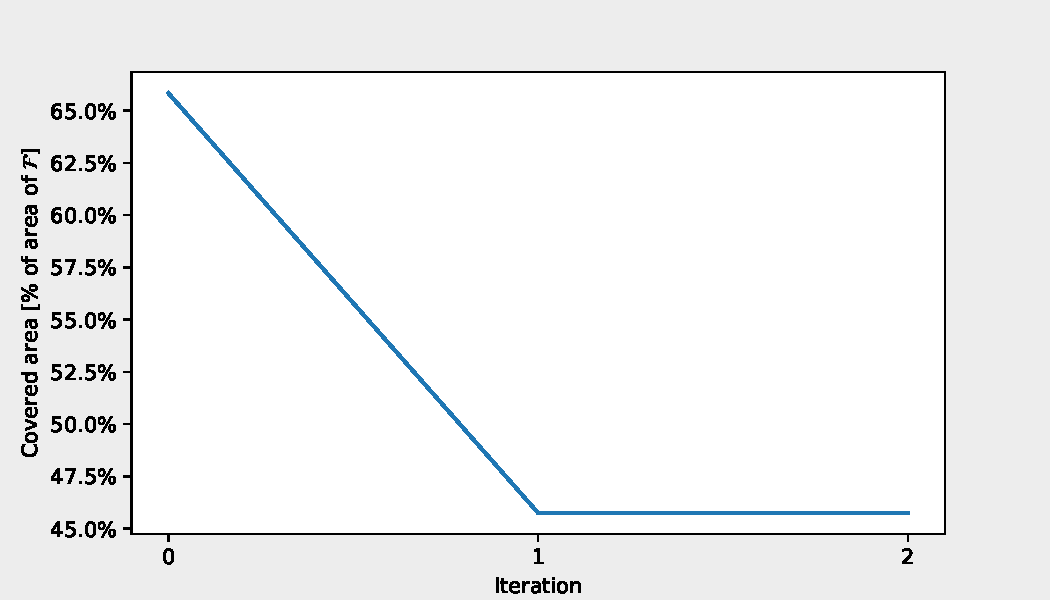
\includegraphics[width=\textwidth]{figs/tinyworld2_3_agnt_k_1_1_k_2_1_area_traj.pdf}
    \caption{Coverage evolution for 3 agents in the Tinyworld2 environment with $k_{1} = k_{2} = 1$ (active dispersion).}
    \label{fig:3_agnt_tw2_k_1_1_a_traj}
  \end{subfigure}%
  ~ 
  \begin{subfigure}[t]{0.5\textwidth}
    \centering
    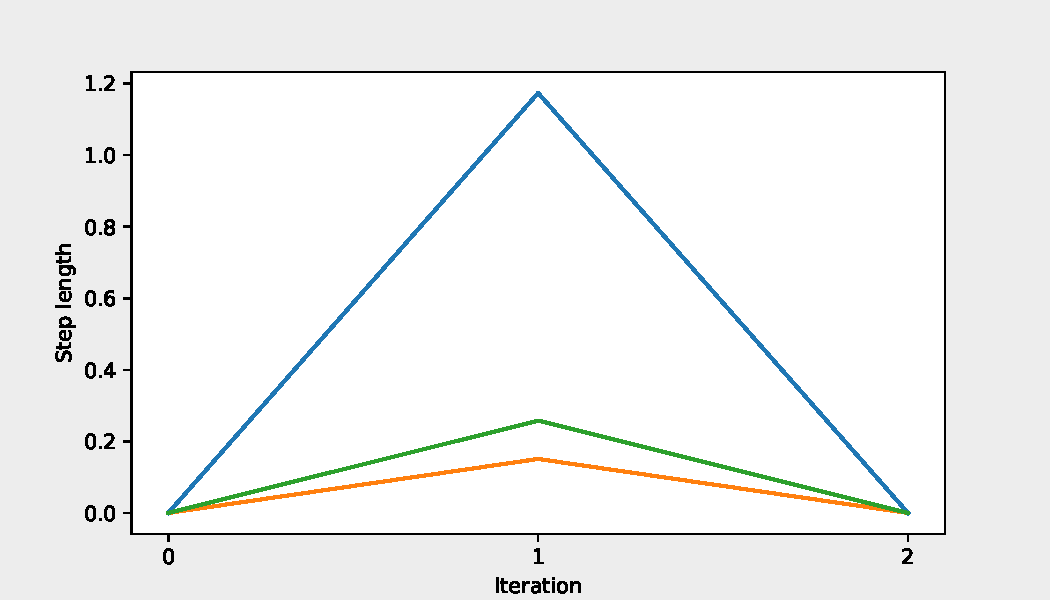
\includegraphics[width=\textwidth]{figs/tinyworld2_3_agnt_k_1_1_k_2_1_step_traj.pdf}
    \caption{Step length evolution for 3 agents in the Tinyworld2 environment with $k_{1} = k_{2} = 1$ (active dispersion).}
    \label{fig:3_agnt_tw2_k_1_1_s_traj}
  \end{subfigure}
  \caption{Coverage percentage and step length evolution for 3 agents in the Tinyworld2 environment when active dispersion is used.}
  \label{fig:3_agnt_tw2_evolution_active}
\end{figure}

\begin{figure}[H]
  \centering
  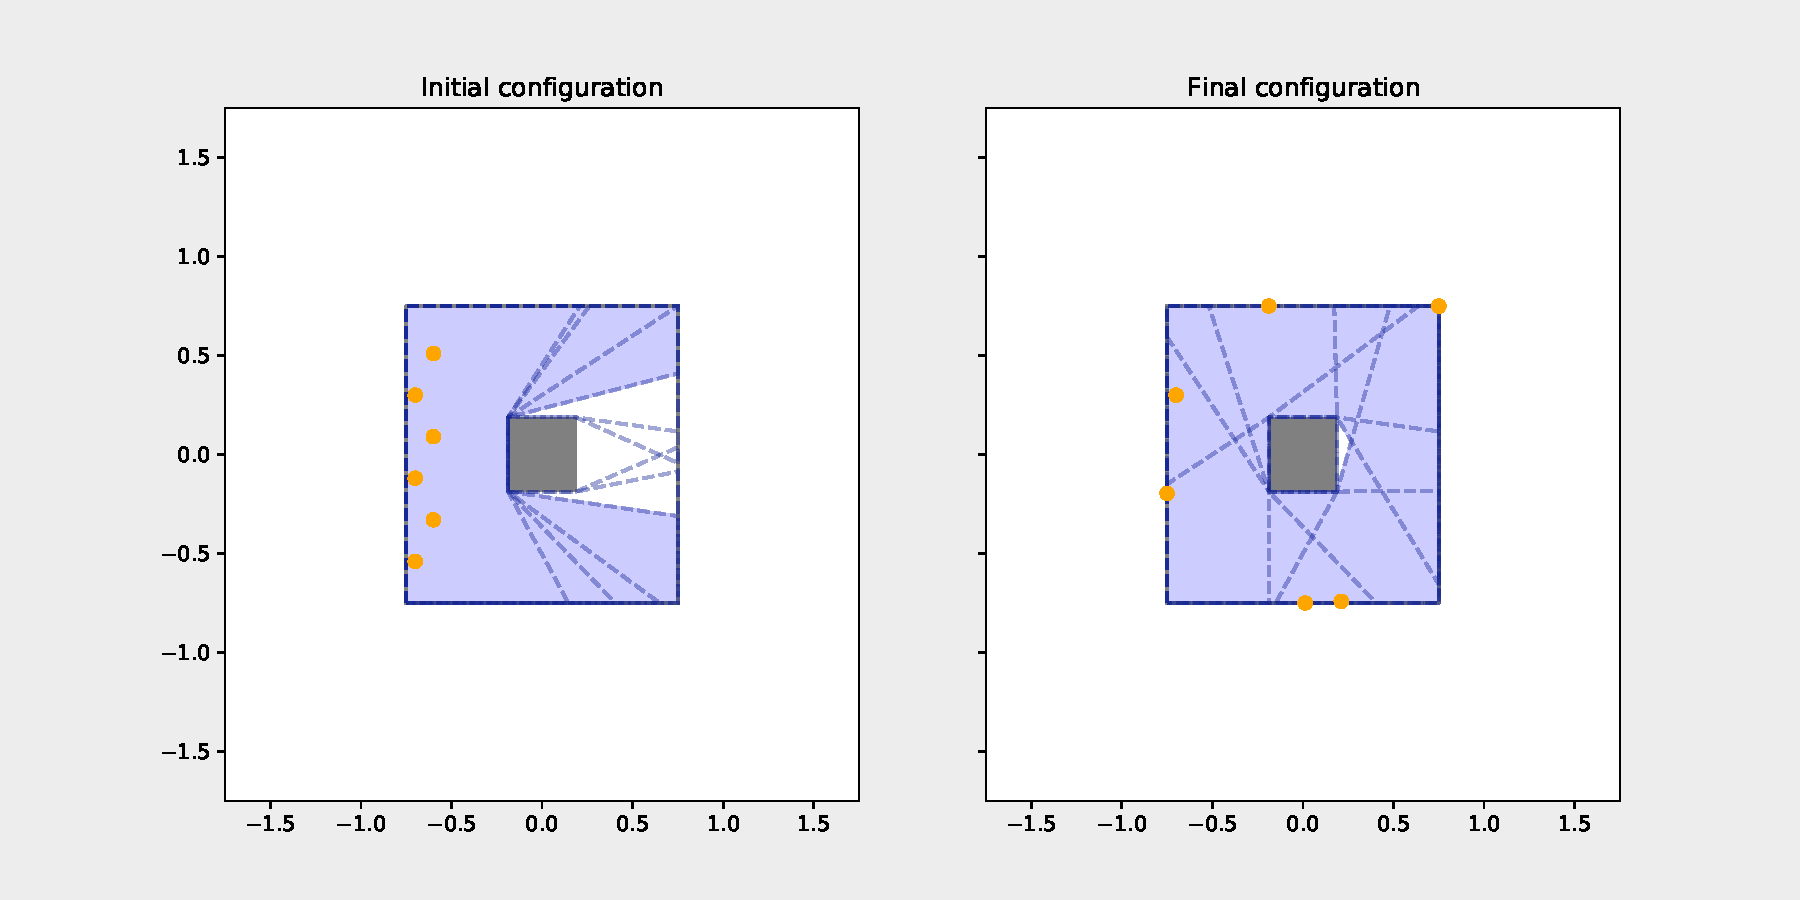
\includegraphics[width=\textwidth]{figs/tinyworld2_6_agnt_k_1_0_k_2_1_distr.pdf}
  \caption{Inital and final configuration of 6 agents in the Tinyworld2 environment with $k_{1} = 0$ (no active dispersion).}
  \label{fig:6_agnt_tw2_k_1_0_distr}
\end{figure}
\begin{figure}[H]
  \centering
  \begin{subfigure}[t]{0.5\textwidth}
    \centering
    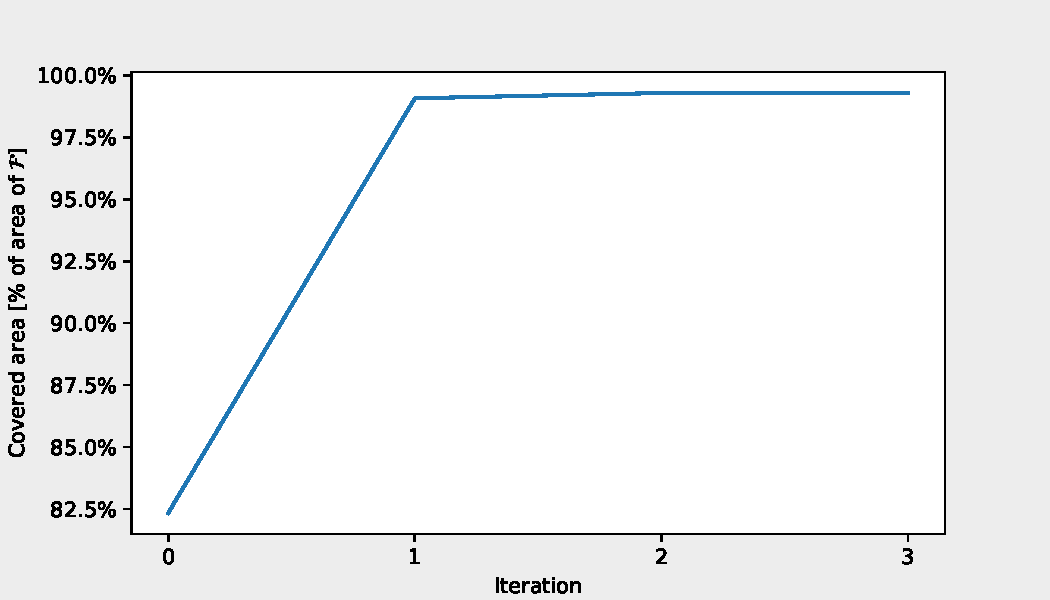
\includegraphics[width=\textwidth]{figs/tinyworld2_6_agnt_k_1_0_k_2_1_area_traj.pdf}
    \caption{Coverage evolution for 6 agents in the Tinyworld2 environment with $k_{1} = 0$ (no active dispersion).}
    \label{fig:6_agnt_tw2_k_1_0_a_traj}
  \end{subfigure}%
  ~ 
  \begin{subfigure}[t]{0.5\textwidth}
    \centering
    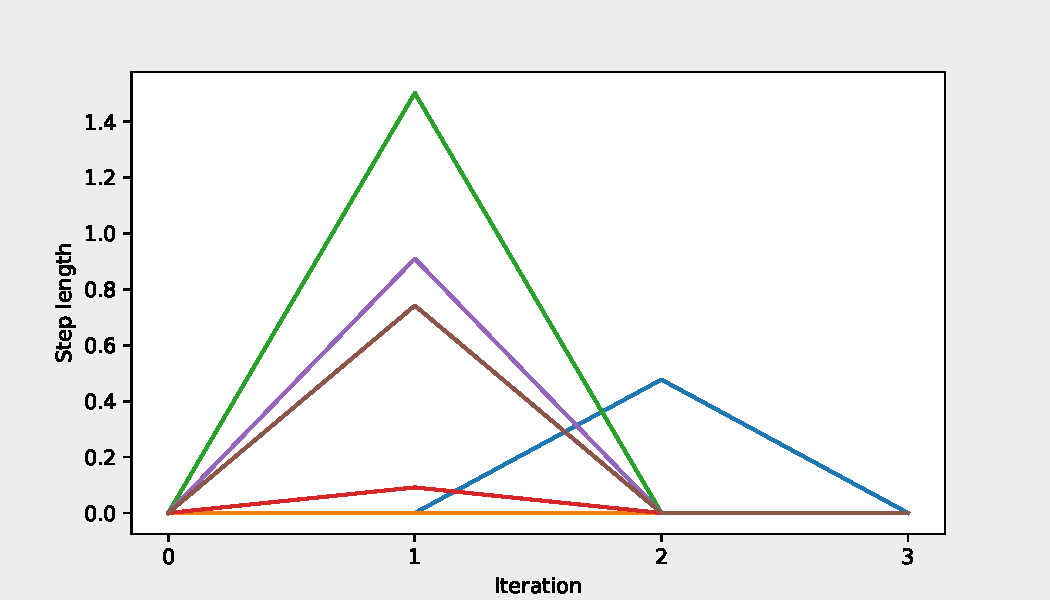
\includegraphics[width=\textwidth]{figs/tinyworld2_6_agnt_k_1_0_k_2_1_step_traj.pdf}
    \caption{Step length evolution for 6 agents in the Tinyworld2 environment with $k_{1} = 0$ (no active dispersion).}
    \label{fig:6_agnt_tw2_k_1_0_s_traj}
  \end{subfigure}
  \caption{Coverage percentage and step length evolution for 6 agents in the Tinyworld2 environment when active dispersion is not applied.}
  \label{fig:6_agnt_tw2_evolution}
\end{figure}

\begin{figure}[H]
  \centering
  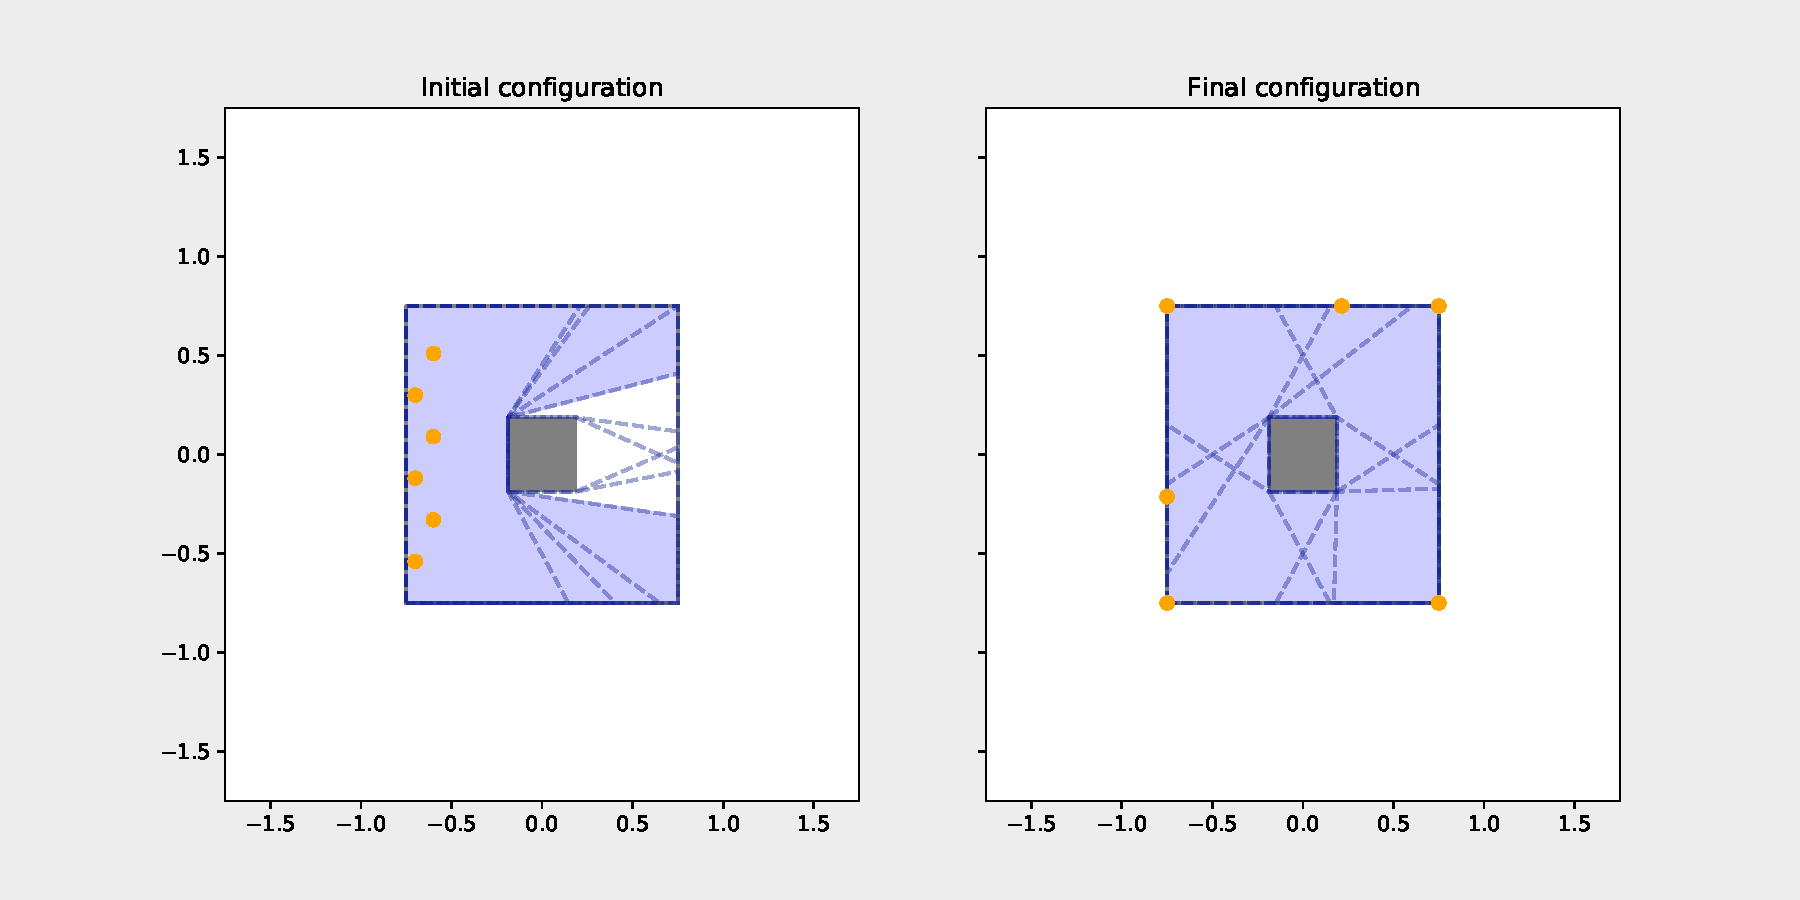
\includegraphics[width=\textwidth]{figs/tinyworld2_6_agnt_k_1_1_k_2_1_distr.pdf}
  \caption{Inital and final configuration of 6 agents in the Tinyworld2 environment with $k_{1} = k_{2} = 1$ (active dispersion).}
  \label{fig:6_agnt_tw2_k_1_1_k_2_1_distr}
\end{figure}
\begin{figure}[H]
  \centering
  \begin{subfigure}[t]{0.5\textwidth}
    \centering
    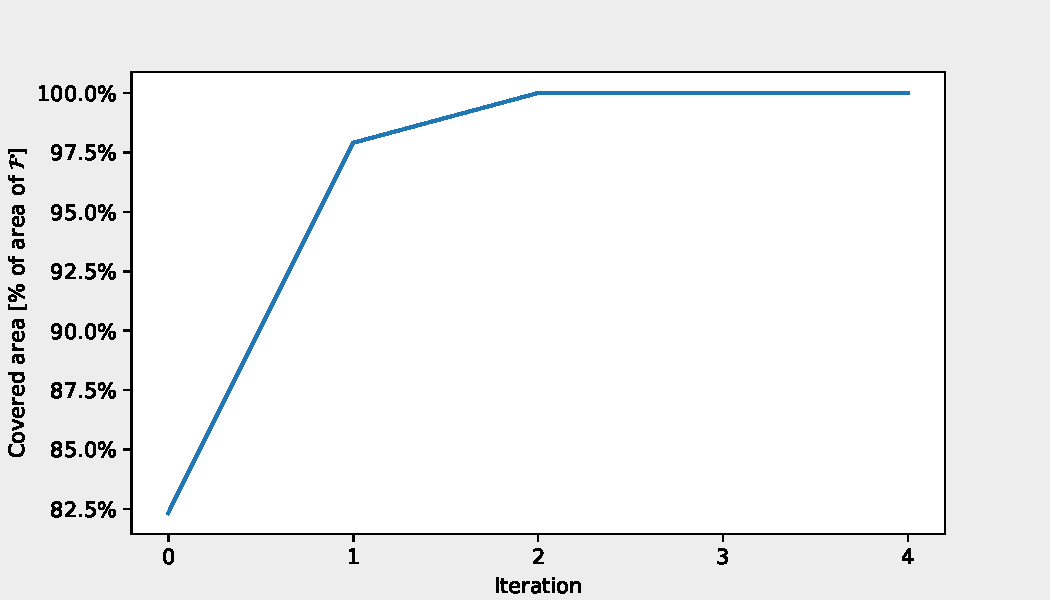
\includegraphics[width=\textwidth]{figs/tinyworld2_6_agnt_k_1_1_k_2_1_area_traj.pdf}
    \caption{Coverage evolution for 6 agents in the Tinyworld2 environment with $k_{1} = k_{1} = 1$ (active dispersion).}
    \label{fig:6_agnt_tw2_k_1_1_a_traj}
  \end{subfigure}%
  ~ 
  \begin{subfigure}[t]{0.5\textwidth}
    \centering
    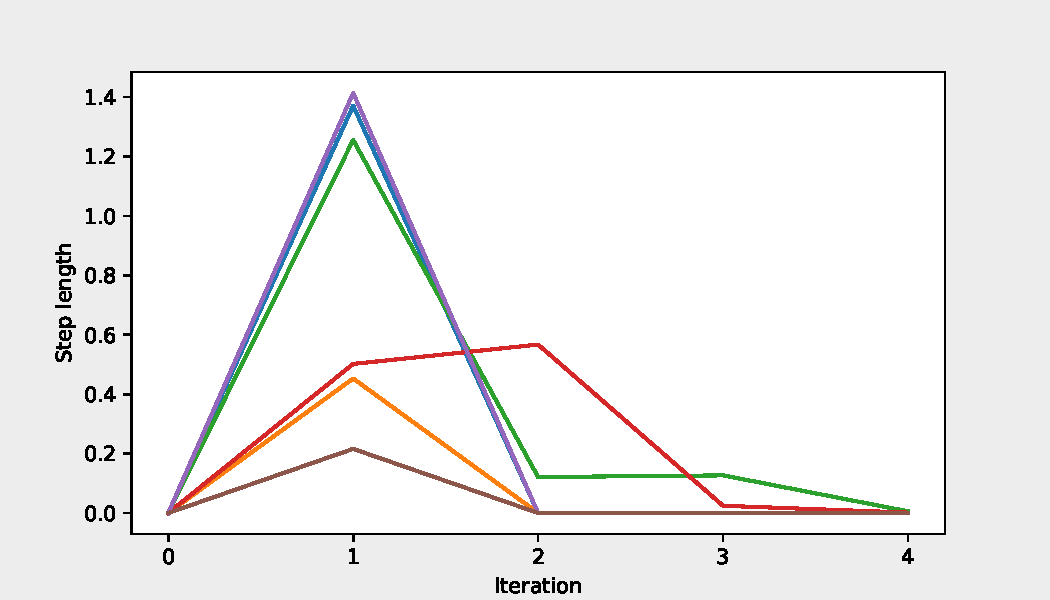
\includegraphics[width=\textwidth]{figs/tinyworld2_6_agnt_k_1_1_k_2_1_step_traj.pdf}
    \caption{Step length evolution for 6 agents in the Tinyworld2 environment with $k_{1} = k_{2} = 1$ (active dispersion).}
    \label{fig:6_agnt_tw2_k_1_1_s_traj}
  \end{subfigure}
  \caption{Coverage percentage and step length evolution for 6 agents in the Tinyworld2 environment when active dispersion is applied.}
  \label{fig:6_agnt_tw2_evolution_active}
\end{figure}

\clearpage
\subsection{Rectworld}\label[secc]{rectworld}
The Rectworld is constructed to examine the behavior of Algorithm \ref{alg:alg1} for a larger mission space. Simulations are performed
for swarms of 3, 6 and 15 agents.

%\Crefrange{fig:3_agnt_bw_k_1_0_k_2_1_distr}{fig:3_agnt_bw_evolution}, \Crefrange{fig:6_agnt_bw_k_1_0_k_2_1_distr}{fig:6_agnt_bw_evolution}
%and \Crefrange{fig:15_agnt_bw_k_1_0_k_2_1_distr}{fig:15_agnt_bw_evolution} show the results of simulating without active dispersion ($k_{1} = 0$) for 3, 6 and 15
%agents respectively.
%
%\Crefrange{fig:3_agnt_bw_k_1_1_k_2_1_distr}{fig:3_agnt_bw_evolution_active}, \Crefrange{fig:6_agnt_bw_k_1_1_k_2_1_distr}{fig:6_agnt_bw_evolution_active}
%and \Crefrange{fig:15_agnt_bw_k_1_1_k_2_1_distr}{fig:15_agnt_bw_evolution_active} show the results of simulating with active dispersion ($k_{1} = k_{2} = 1$) for 3, 6 and 15
%agents respectively.

\begin{figure}[H]
  \centering
  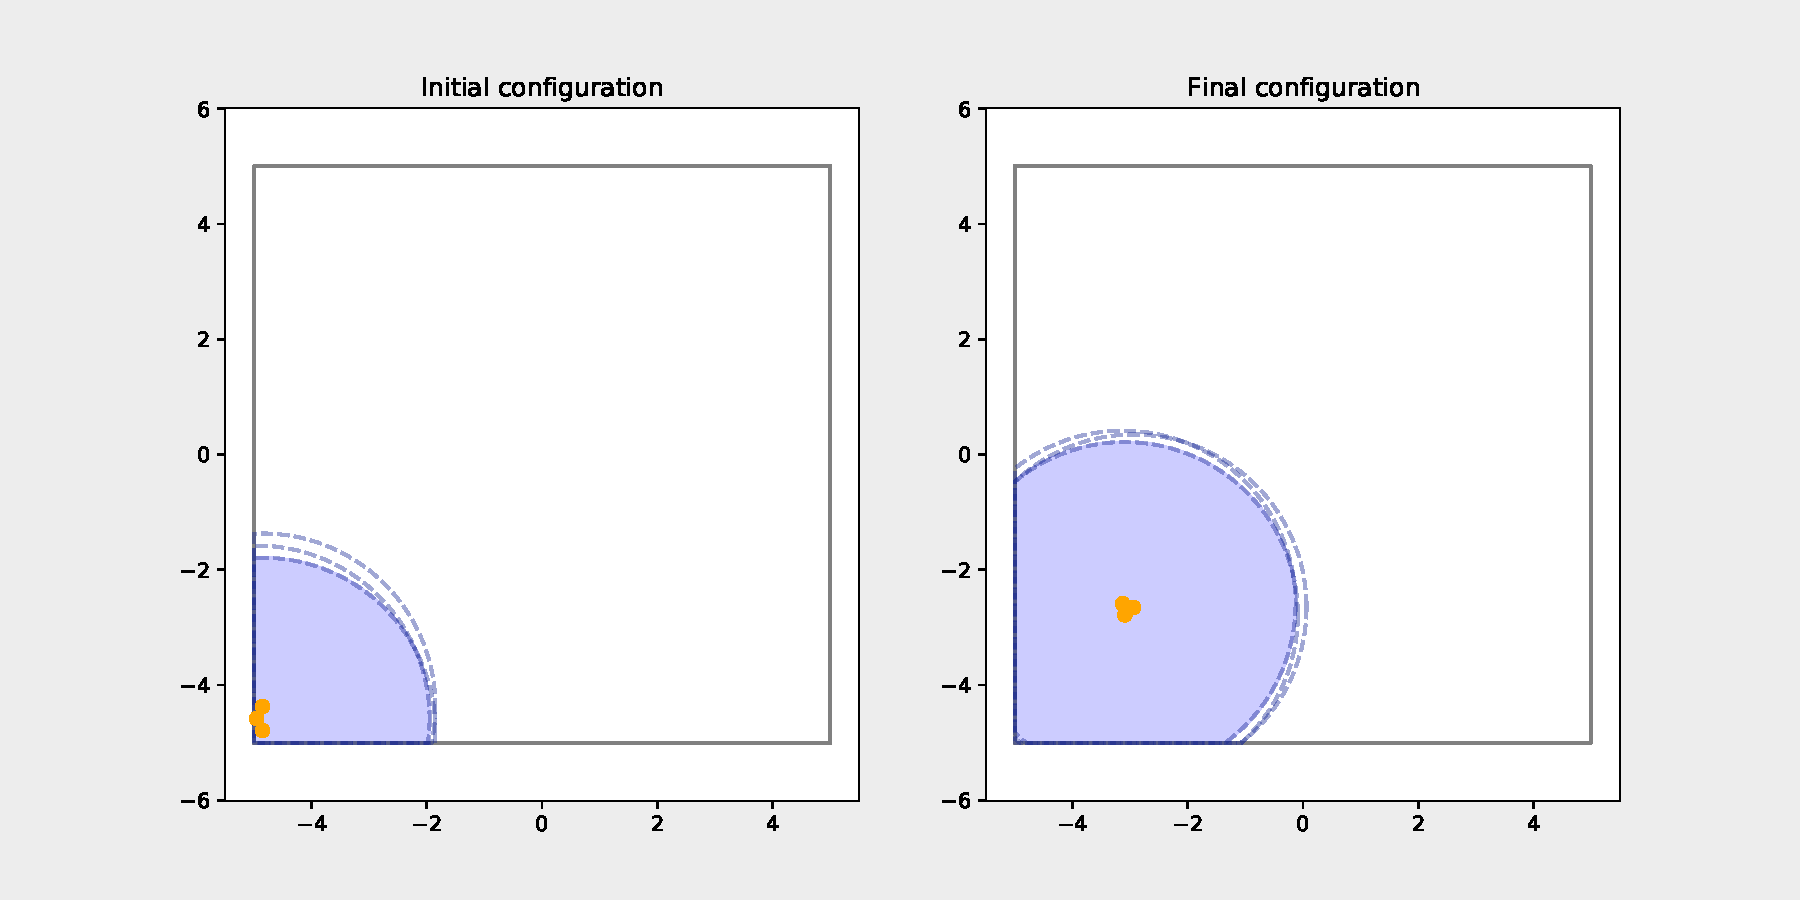
\includegraphics[width=\textwidth]{figs/bigworld_3_agnt_k_1_0_k_2_1_distr.pdf}
  \caption{Initial and final configuration of 3 agents in the Rectworld environment with $k_{1} = 0$ (no active dispersion).}
  \label{fig:3_agnt_bw_k_1_0_k_2_1_distr}
\end{figure}
\begin{figure}[H]
  \centering
  \begin{subfigure}[t]{0.5\textwidth}
    \centering
    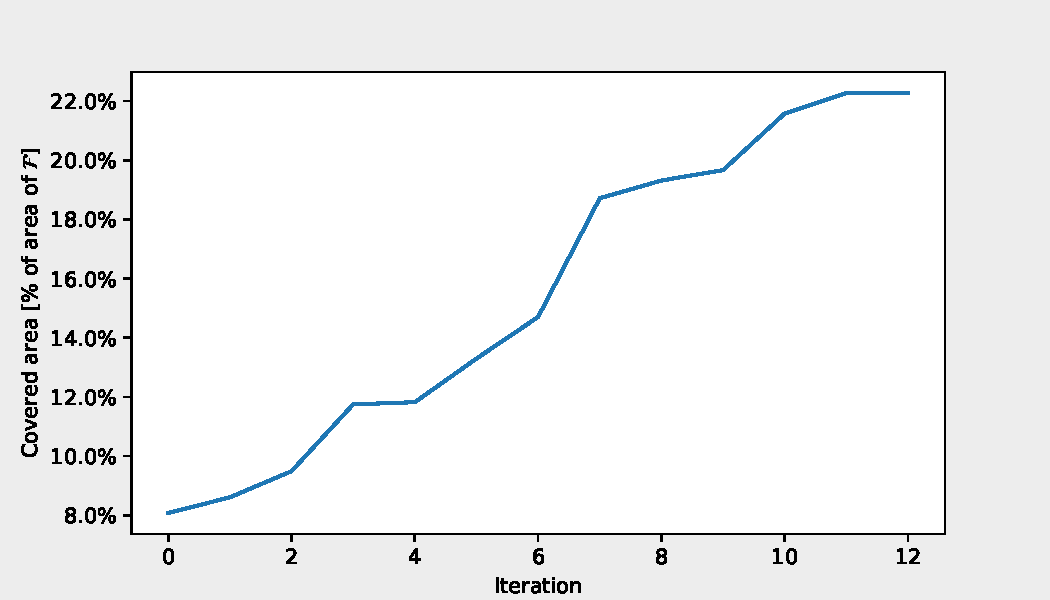
\includegraphics[width=\textwidth]{figs/bigworld_3_agnt_k_1_0_k_2_1_area_traj.pdf}
    \caption{Coverage evolution for 3 agents in the Rectworld environment with $k_{1} = 0$ (no active dispersion).}
    \label{fig:3_agnt_bw_k_1_0_a_traj}
  \end{subfigure}%
  ~ 
  \begin{subfigure}[t]{0.5\textwidth}
    \centering
    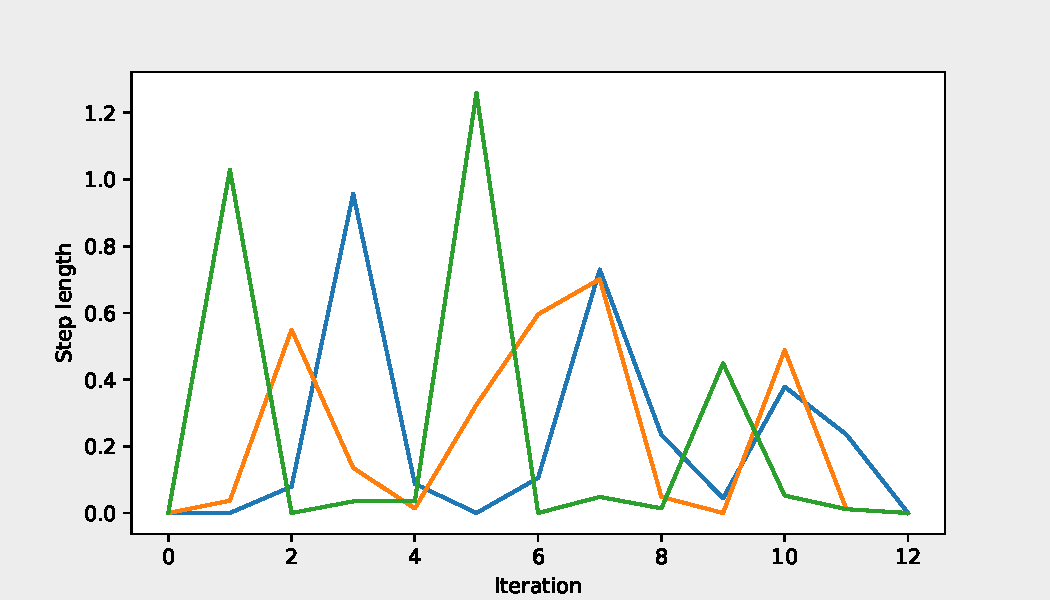
\includegraphics[width=\textwidth]{figs/bigworld_3_agnt_k_1_0_k_2_1_step_traj.pdf}
    \caption{Step length evolution for 3 agents in the Rectworld environment with $k_{1} = 0$ (no active dispersion).}
    \label{fig:3_agnt_bw_k_1_0_s_traj}
  \end{subfigure}
  \caption{Coverage percentage and step length evolution for 3 agents in the Rectworld environment when no active dispersion is used.}
  \label{fig:3_agnt_bw_evolution}
\end{figure}


\begin{figure}[H]
  \centering
  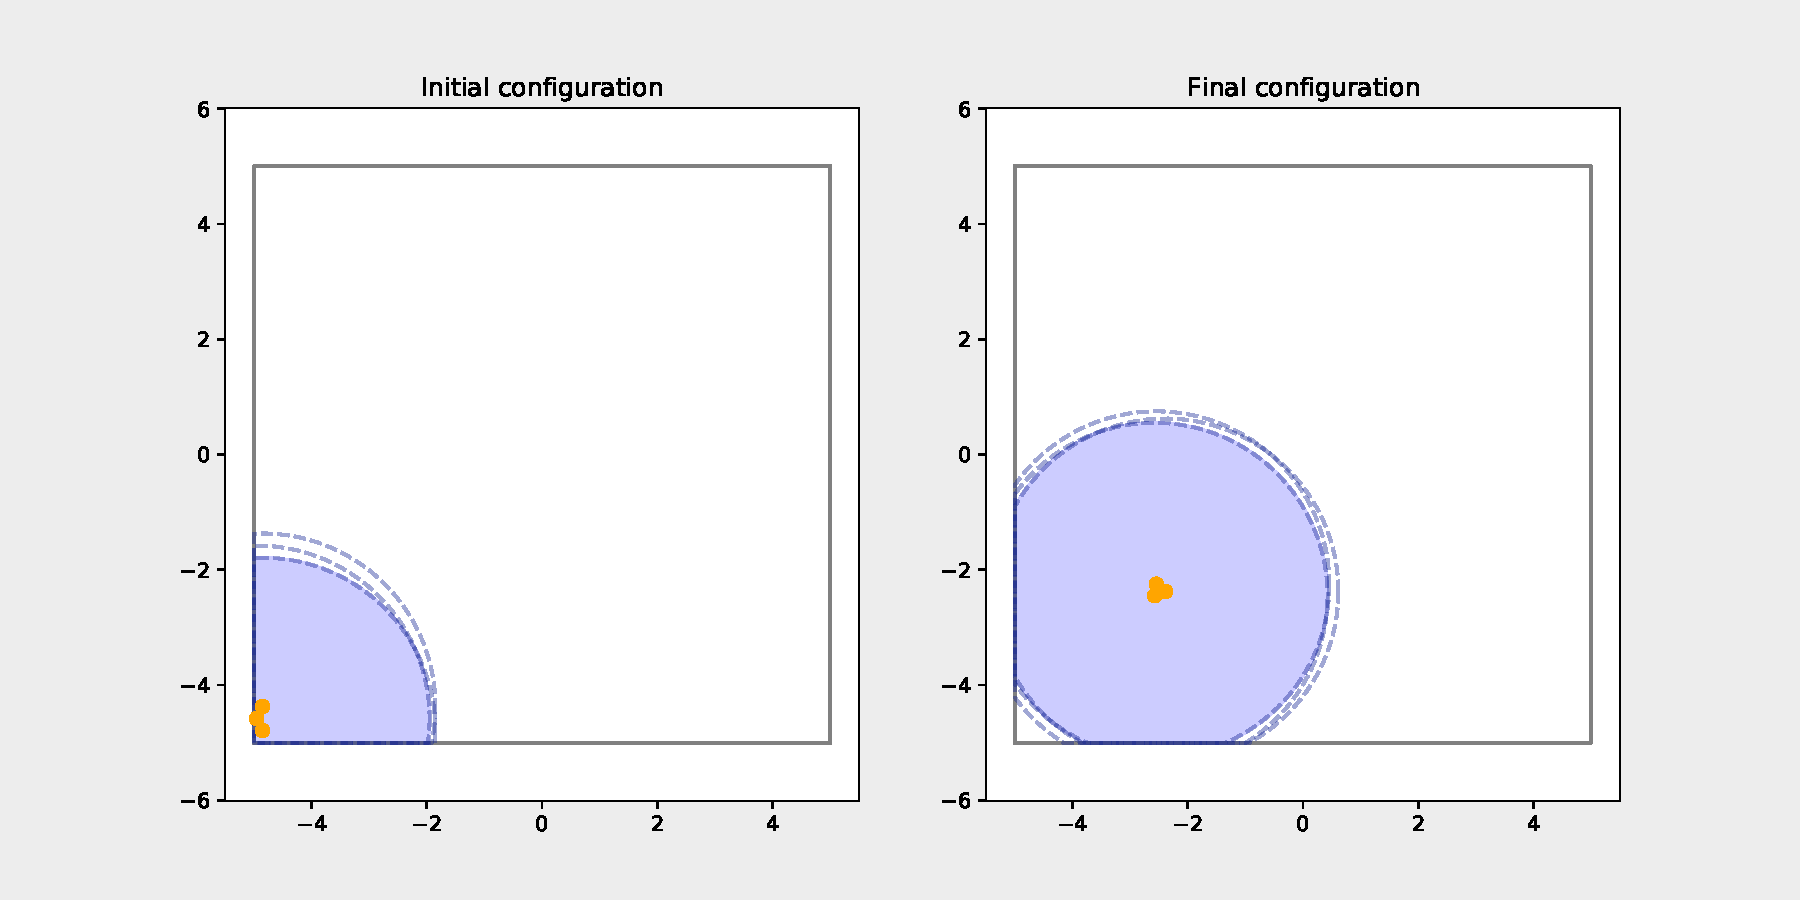
\includegraphics[width=\textwidth]{figs/bigworld_3_agnt_k_1_1_k_2_1_distr.pdf}
  \caption{Initial and final configuration of 3 agents in the Rectworld environment with $k_{1} = k_{2} = 1$ (active dispersion).}
  \label{fig:3_agnt_bw_k_1_1_k_2_1_distr}
\end{figure}
\begin{figure}[H]
  \centering
  \begin{subfigure}[t]{0.5\textwidth}
    \centering
    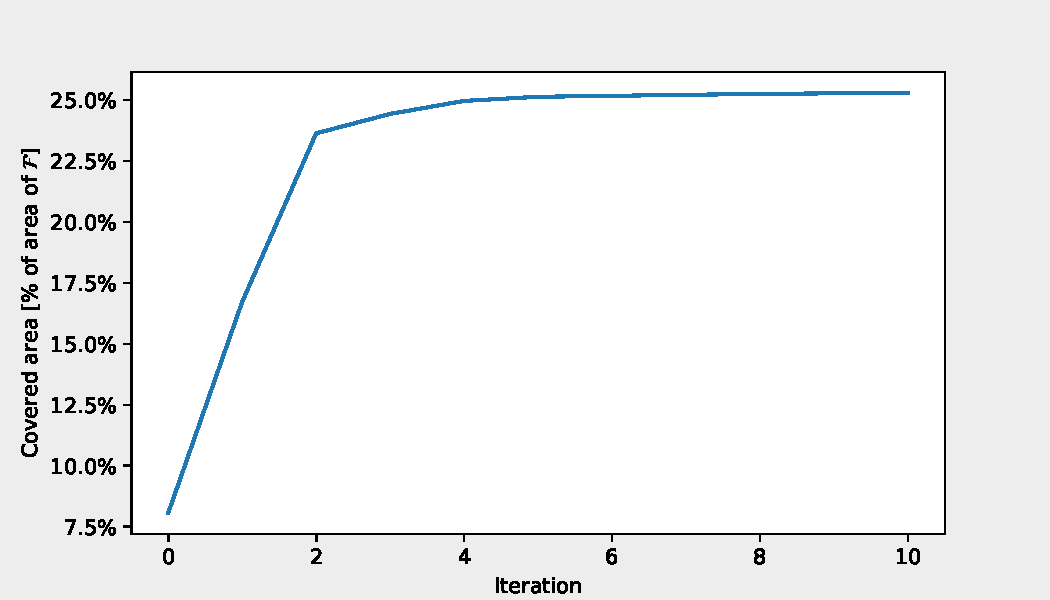
\includegraphics[width=\textwidth]{figs/bigworld_3_agnt_k_1_1_k_2_1_area_traj.pdf}
    \caption{Coverage evolution for 3 agents in the Rectworld environment with $k_{1} = k_{1} = 1$ (active dispersion).}
    \label{fig:3_agnt_bw_k_1_1_a_traj}
  \end{subfigure}%
  ~ 
  \begin{subfigure}[t]{0.5\textwidth}
    \centering
    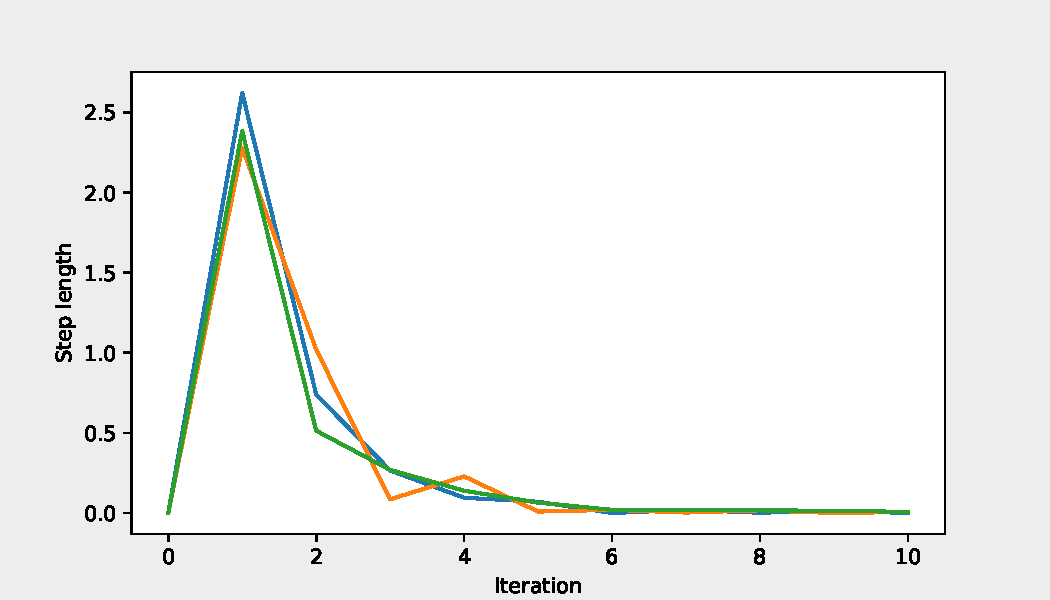
\includegraphics[width=\textwidth]{figs/bigworld_3_agnt_k_1_1_k_2_1_step_traj.pdf}
    \caption{Step length evolution for 3 agents in the Rectworld environment with $k_{1} = k_{1} = 1$ (active dispersion).}
    \label{fig:3_agnt_bw_k_1_1_s_traj}
  \end{subfigure}
  \caption{Coverage percentage and step length evolution for 3 agents in the Rectworld environment when active dispersion is used.}
  \label{fig:3_agnt_bw_evolution_active}
\end{figure}

%%%

\begin{figure}[H]
  \centering
  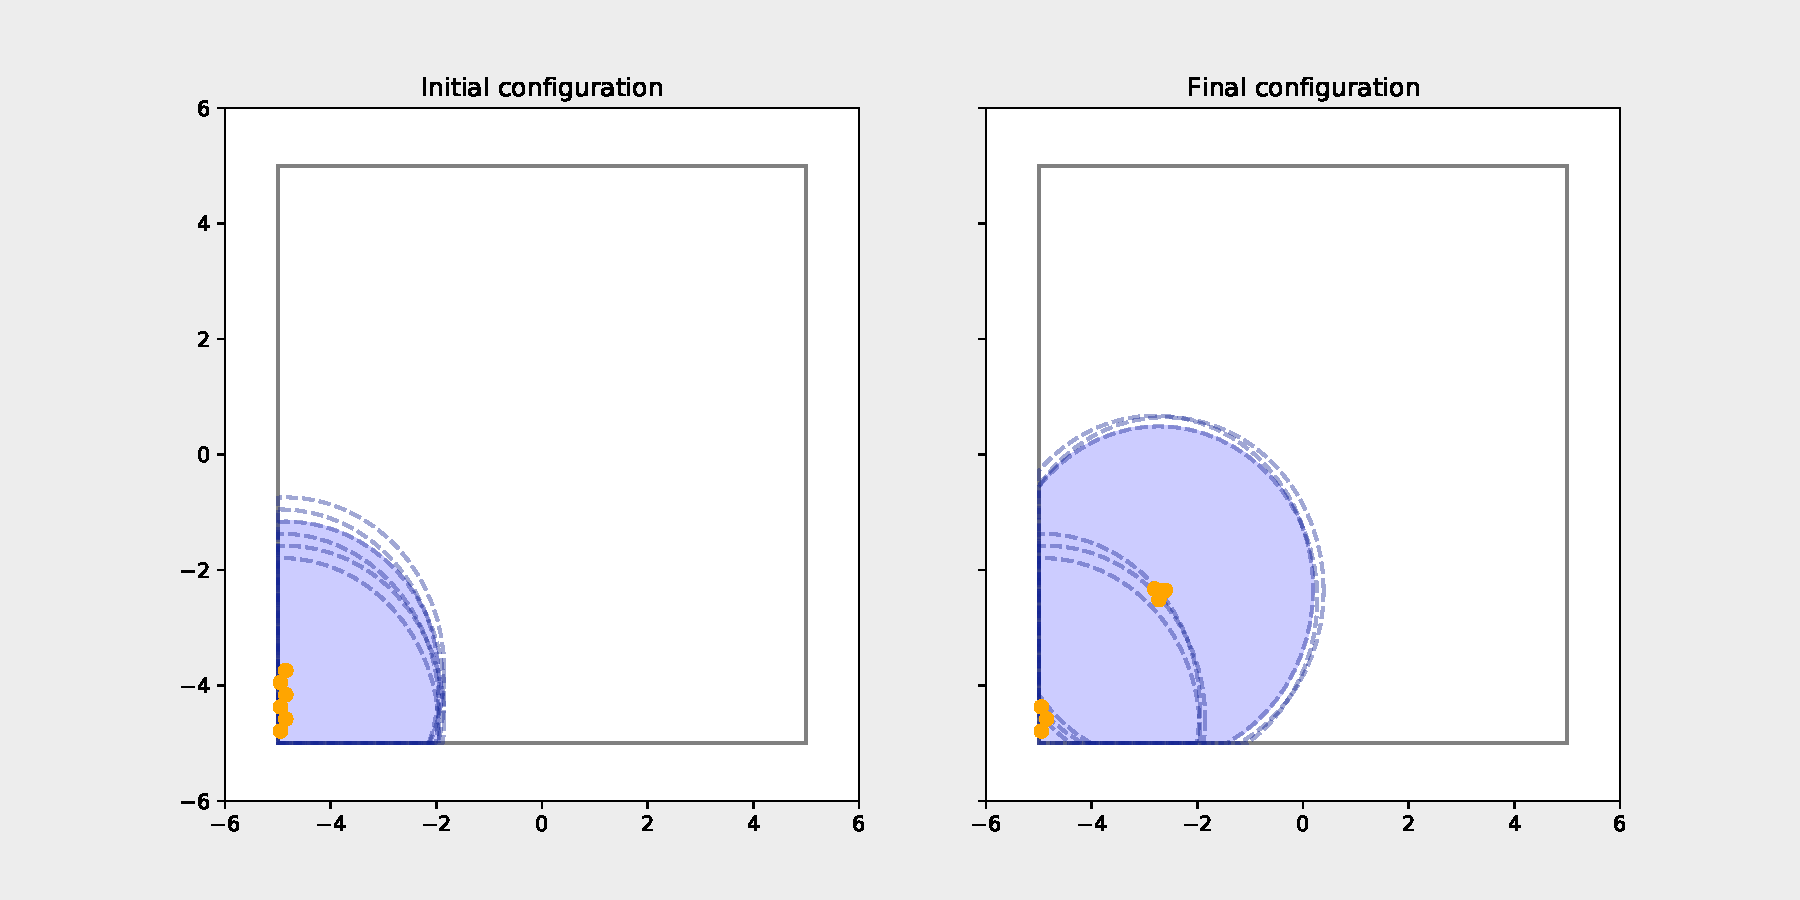
\includegraphics[width=\textwidth]{figs/bigworld_6_agnt_k_1_0_k_2_1_distr.pdf}
  \caption{Initial and final configuration of 6 agents in the Rectworld environment with $k_{1} = 0$ (no active dispersion).}
  \label{fig:6_agnt_bw_k_1_0_k_2_1_distr}
\end{figure}
\begin{figure}[H]
  \centering
  \begin{subfigure}[t]{0.5\textwidth}
    \centering
    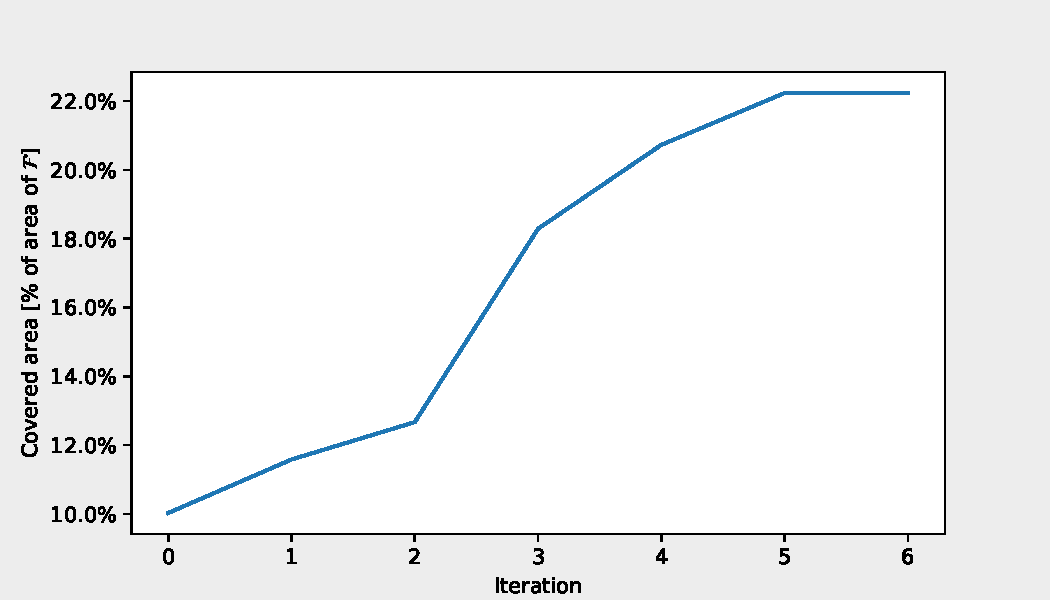
\includegraphics[width=\textwidth]{figs/bigworld_6_agnt_k_1_0_k_2_1_area_traj.pdf}
    \caption{Coverage evolution for 6 agents in the Rectworld environment with $k_{1} = 0$ (no active dispersion).}
    \label{fig:6_agnt_bw_k_1_0_a_traj}
  \end{subfigure}%
  ~ 
  \begin{subfigure}[t]{0.5\textwidth}
    \centering
    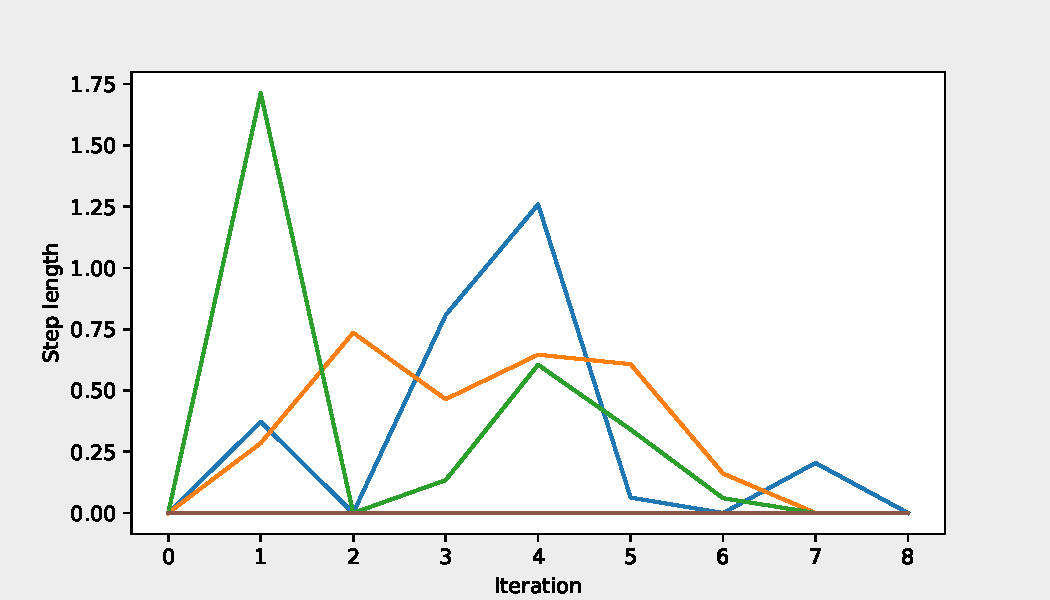
\includegraphics[width=\textwidth]{figs/bigworld_6_agnt_k_1_0_k_2_1_step_traj.pdf}
    \caption{Step length evolution for 6 agents in the Rectworld environment with $k_{1} = 0$ (no active dispersion).}
    \label{fig:6_agnt_bw_k_1_0_s_traj}
  \end{subfigure}
  \caption{Coverage percentage and step length evolution for 6 agents in the Rectworld environment when no active dispersion is used.}
  \label{fig:6_agnt_bw_evolution}
\end{figure}


\begin{figure}[H]
  \centering
  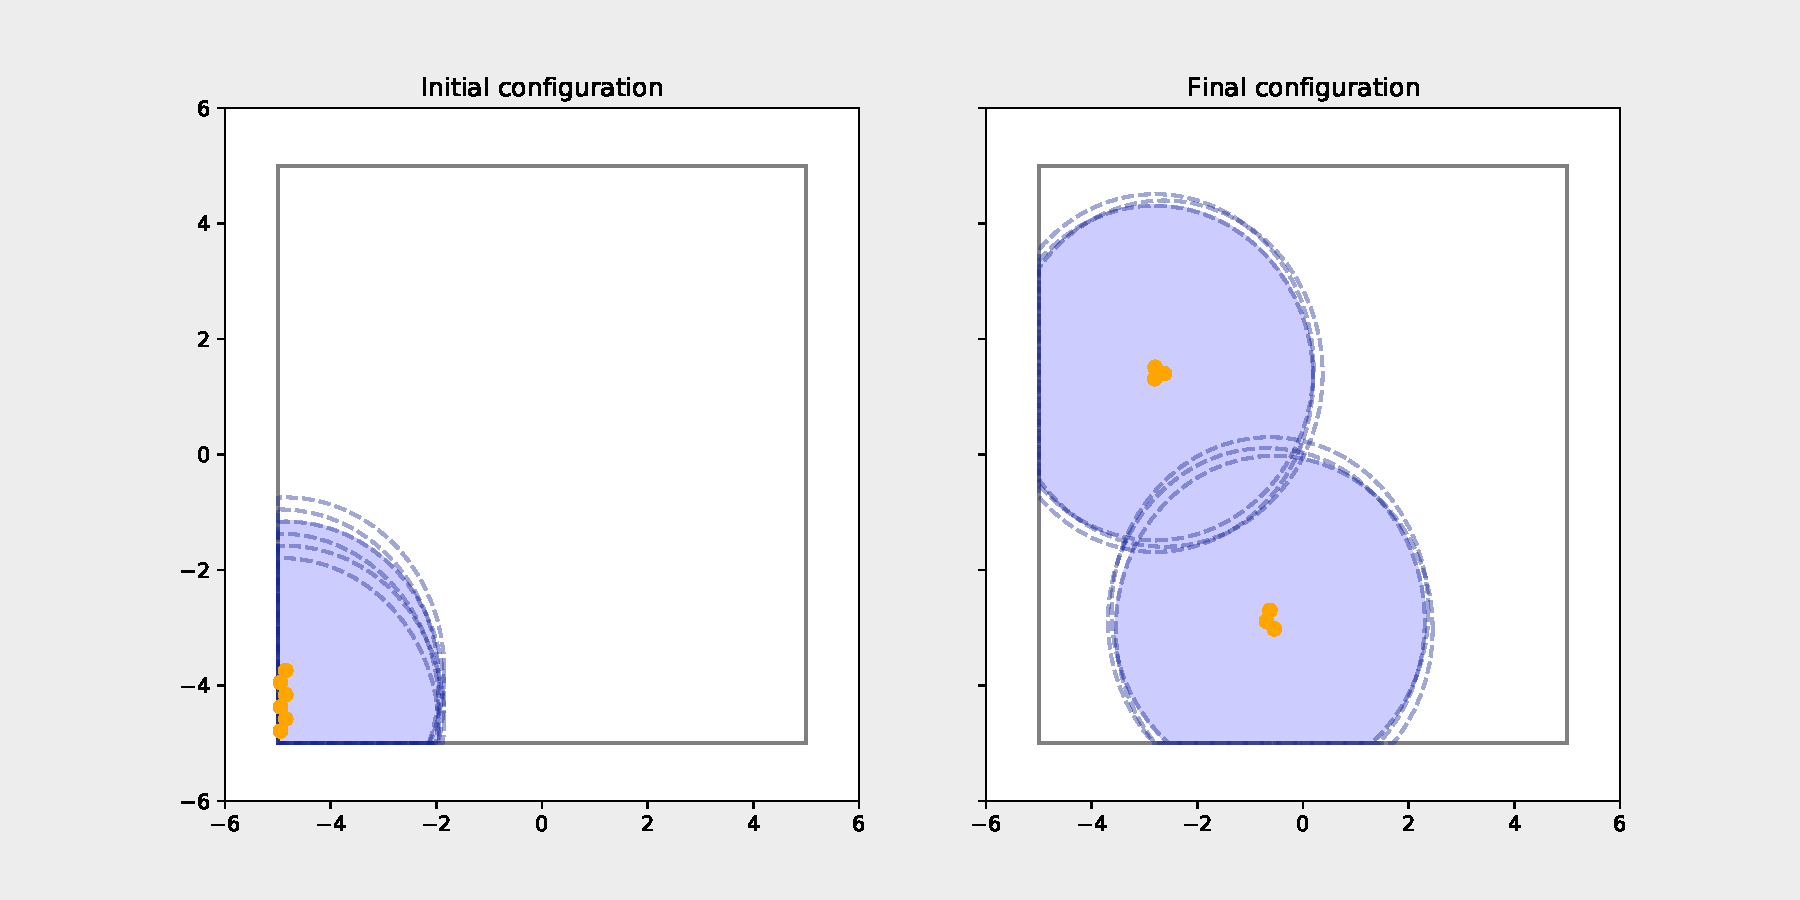
\includegraphics[width=\textwidth]{figs/bigworld_6_agnt_k_1_1_k_2_1_distr.pdf}
  \caption{Initial and final configuration of 6 agents in the Rectworld environment with $k_{1} = k_{2} = 1$ (active dispersion).}
  \label{fig:6_agnt_bw_k_1_1_k_2_1_distr}
\end{figure}
\begin{figure}[H]
  \centering
  \begin{subfigure}[t]{0.5\textwidth}
    \centering
    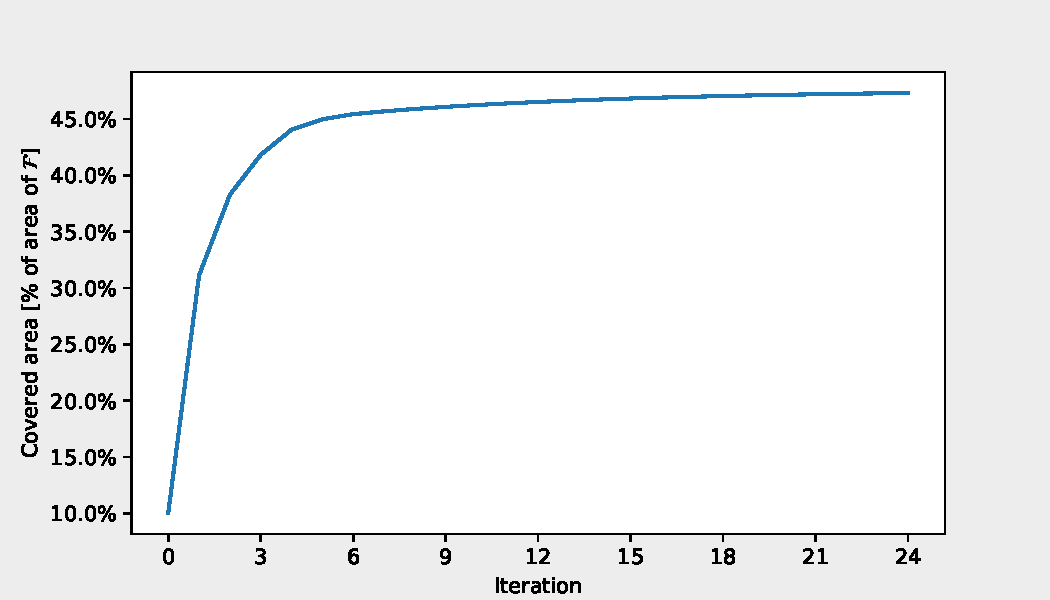
\includegraphics[width=\textwidth]{figs/bigworld_6_agnt_k_1_1_k_2_1_area_traj.pdf}
    \caption{Coverage evolution for 6 agents in the Rectworld environment with $k_{1} = k_{1} = 1$ (active dispersion).}
    \label{fig:6_agnt_bw_k_1_1_a_traj}
  \end{subfigure}%
  ~ 
  \begin{subfigure}[t]{0.5\textwidth}
    \centering
    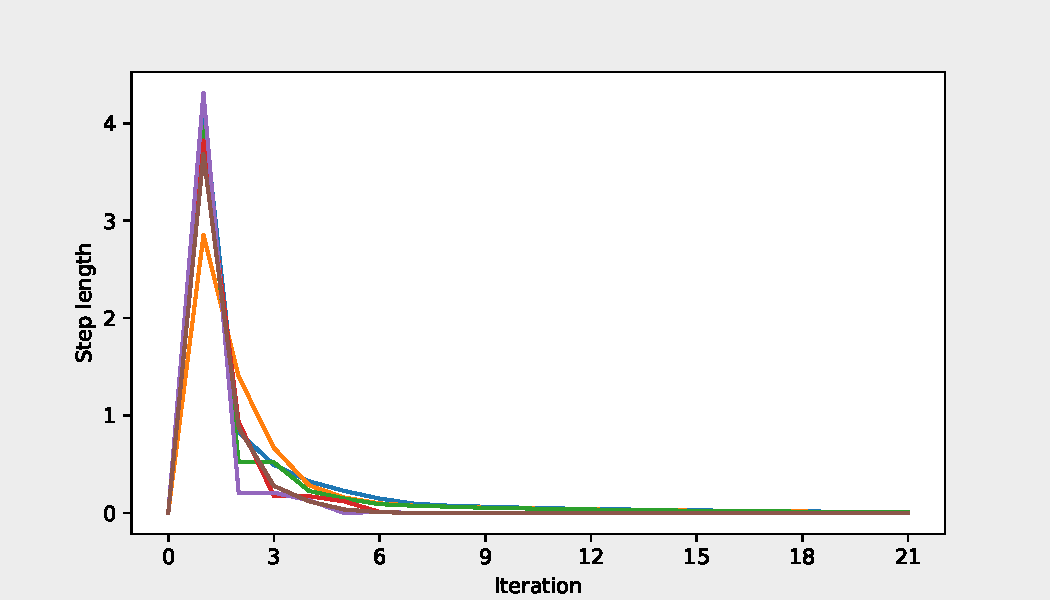
\includegraphics[width=\textwidth]{figs/bigworld_6_agnt_k_1_1_k_2_1_step_traj.pdf}
    \caption{Step length evolution for 6 agents in the Rectworld environment with $k_{1} = k_{1} = 1$ (active dispersion).}
    \label{fig:6_agnt_bw_k_1_1_s_traj}
  \end{subfigure}
  \caption{Coverage percentage and step length evolution for 6 agents in the Rectworld environment when active dispersion is used.}
  \label{fig:6_agnt_bw_evolution_active}
\end{figure}

%%%

\begin{figure}[H]
  \centering
  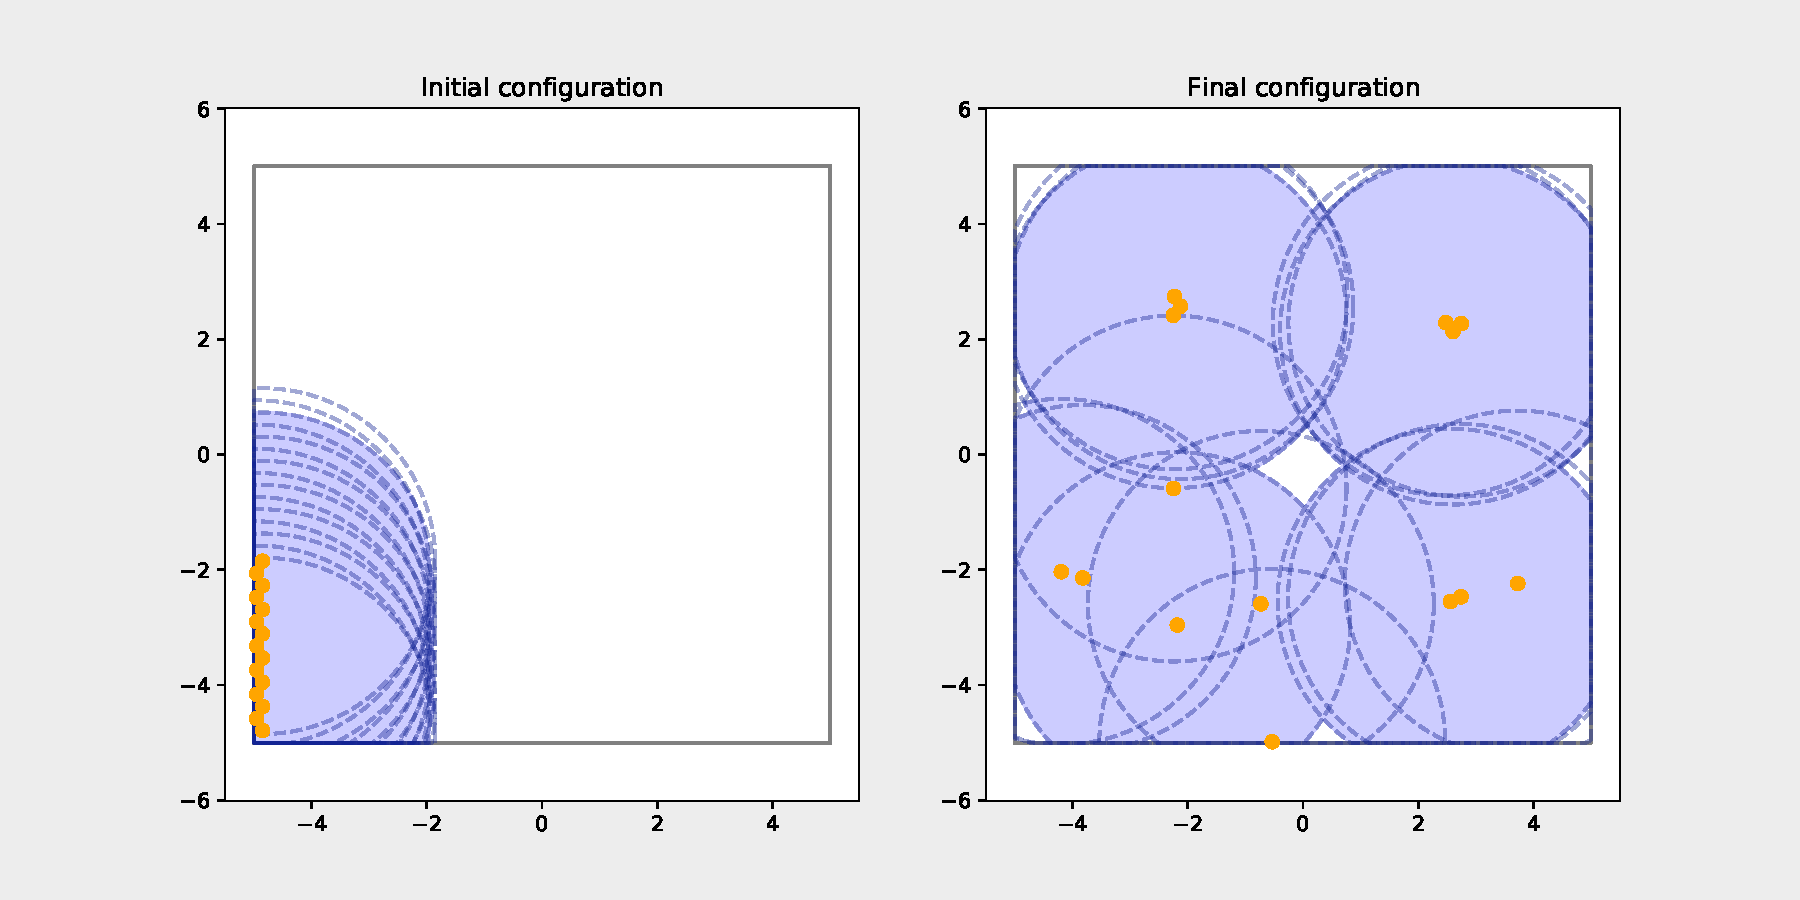
\includegraphics[width=\textwidth]{figs/bigworld_15_agnt_k_1_0_k_2_1_distr.pdf}
  \caption{Initial and final configuration of 15 agents in the Rectworld environment with $k_{1} = 0$ (no active dispersion).}
  \label{fig:15_agnt_bw_k_1_0_k_2_1_distr}
\end{figure}
\begin{figure}[H]
  \centering
  \begin{subfigure}[t]{0.5\textwidth}
    \centering
    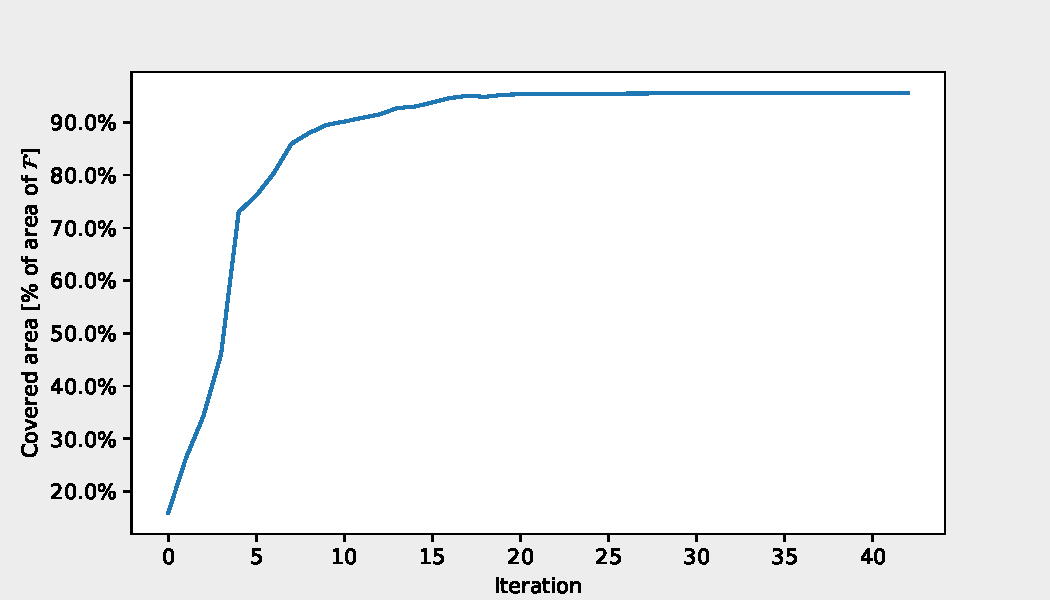
\includegraphics[width=\textwidth]{figs/bigworld_15_agnt_k_1_0_k_2_1_area_traj.pdf}
    \caption{Coverage evolution for 15 agents in the Rectworld environment with $k_{1} = 0$ (no active dispersion).}
    \label{fig:15_agnt_bw_k_1_0_a_traj}
  \end{subfigure}%
  ~ 
  \begin{subfigure}[t]{0.5\textwidth}
    \centering
    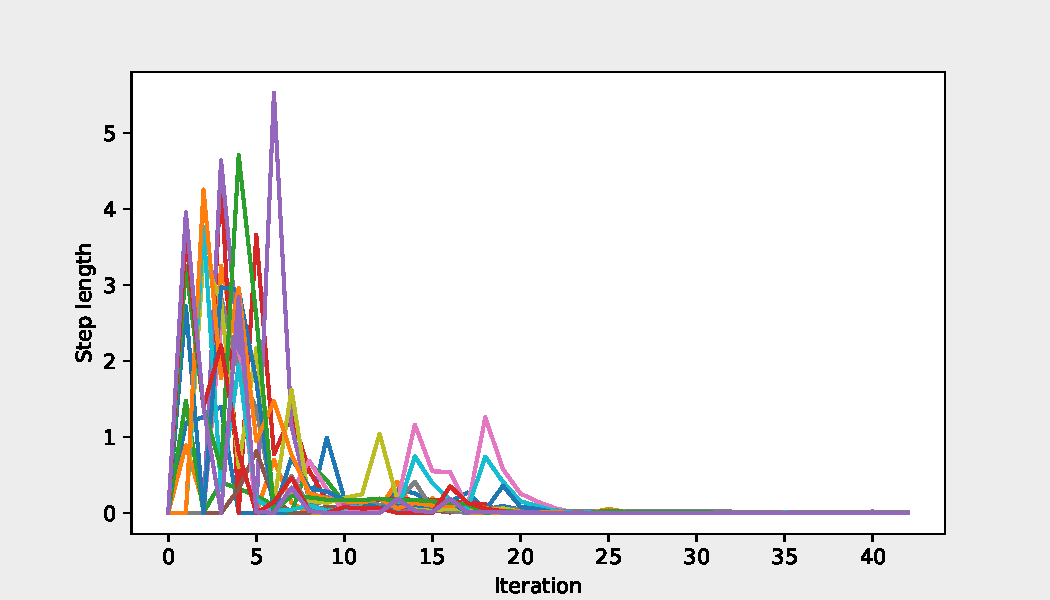
\includegraphics[width=\textwidth]{figs/bigworld_15_agnt_k_1_0_k_2_1_step_traj.pdf}
    \caption{Step length evolution for 15 agents in the Rectworld environment with $k_{1} = 0$ (no active dispersion).}
    \label{fig:15_agnt_bw_k_1_0_s_traj}
  \end{subfigure}
  \caption{Coverage percentage and step length evolution for 15 agents in the Rectworld environment when no active dispersion is used.}
  \label{fig:15_agnt_bw_evolution}
\end{figure}


\begin{figure}[H]
  \centering
  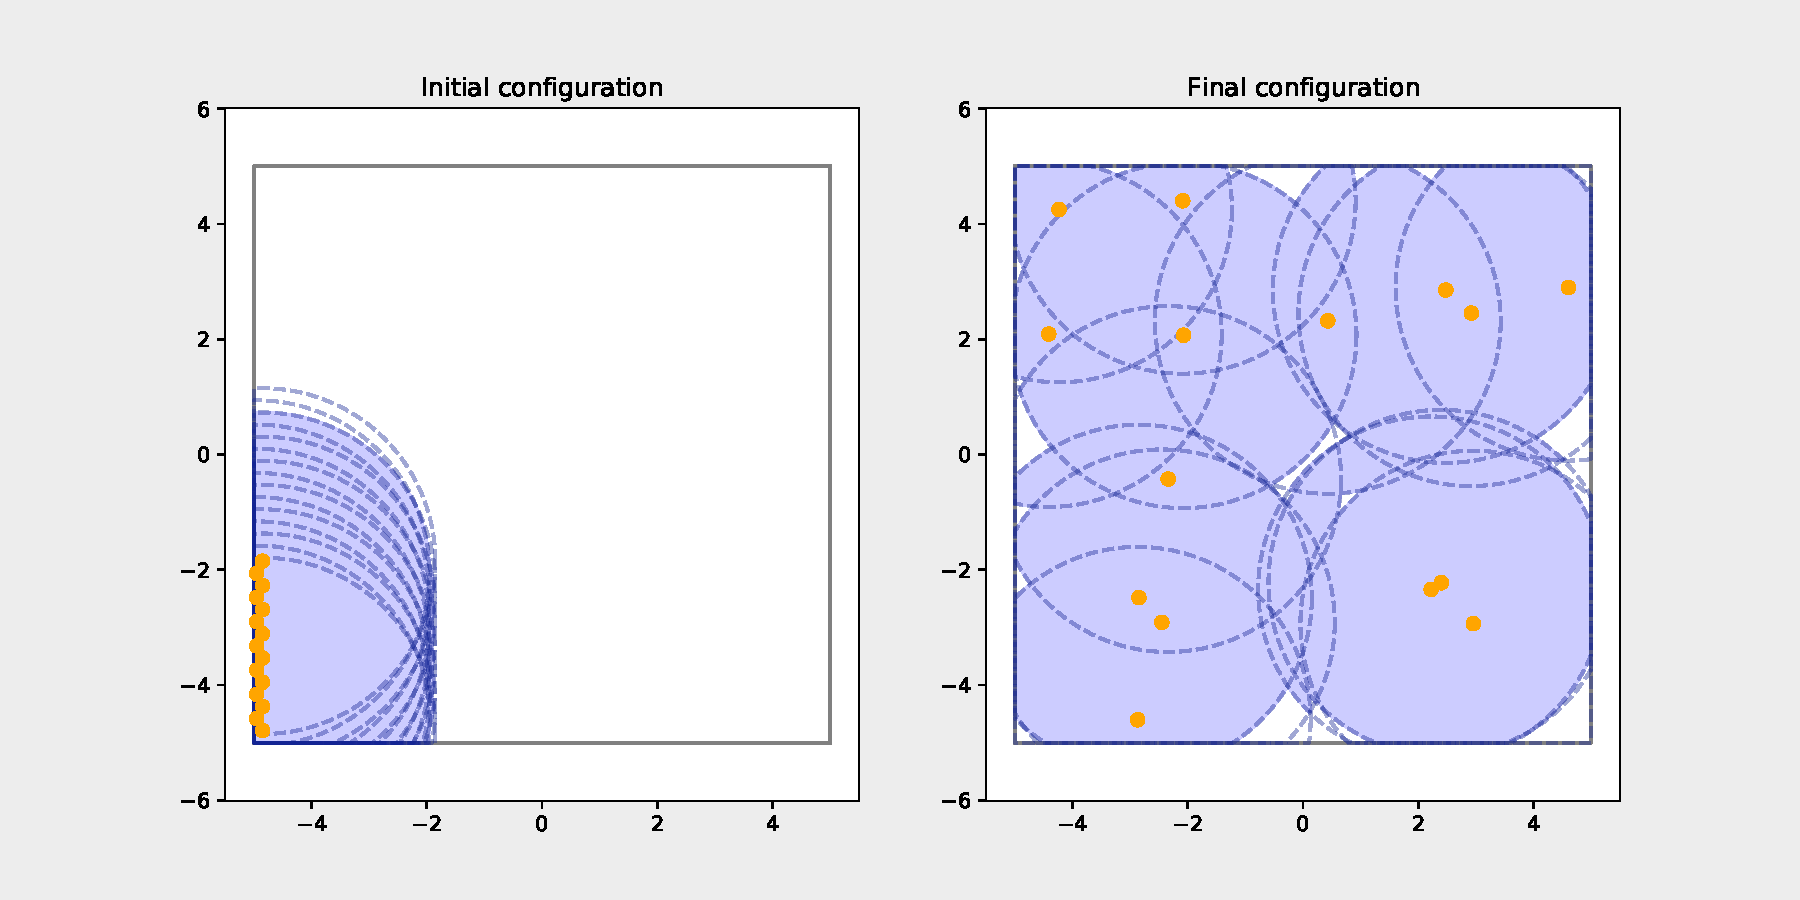
\includegraphics[width=\textwidth]{figs/bigworld_15_agnt_k_1_1_k_2_1_distr.pdf}
  \caption{Initial and final configuration of 15 agents in the Rectworld environment with $k_{1} = k_{2} = 1$ (active dispersion).}
  \label{fig:15_agnt_bw_k_1_1_k_2_1_distr}
\end{figure}
\begin{figure}[H]
  \centering
  \begin{subfigure}[t]{0.5\textwidth}
    \centering
    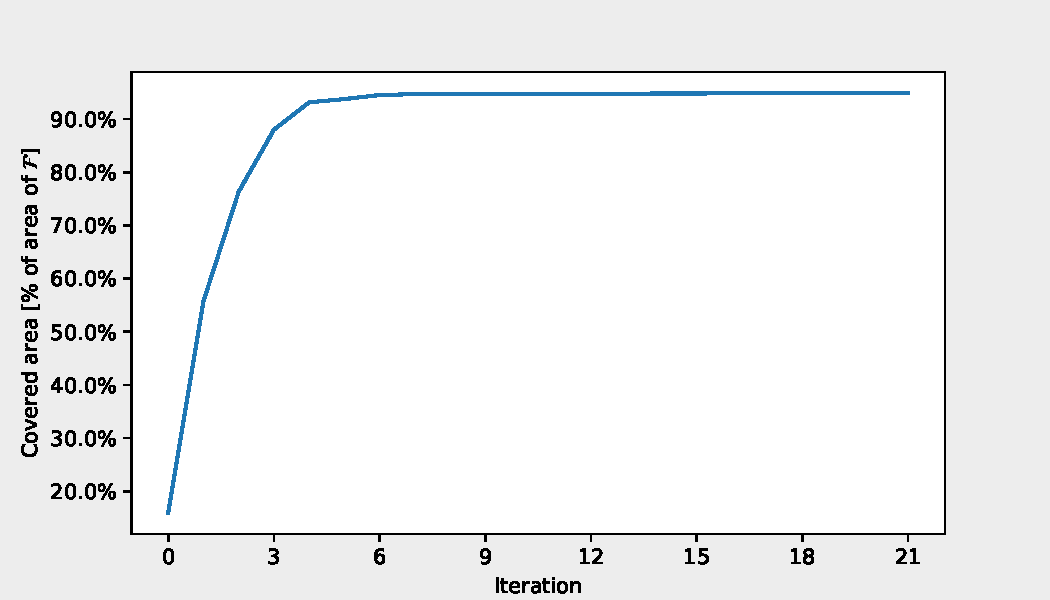
\includegraphics[width=\textwidth]{figs/bigworld_15_agnt_k_1_1_k_2_1_area_traj.pdf}
    \caption{Coverage evolution for 15 agents in the Rectworld environment with $k_{1} = k_{1} = 1$ (active dispersion).}
    \label{fig:15_agnt_bw_k_1_1_a_traj}
  \end{subfigure}%
  ~ 
  \begin{subfigure}[t]{0.5\textwidth}
    \centering
    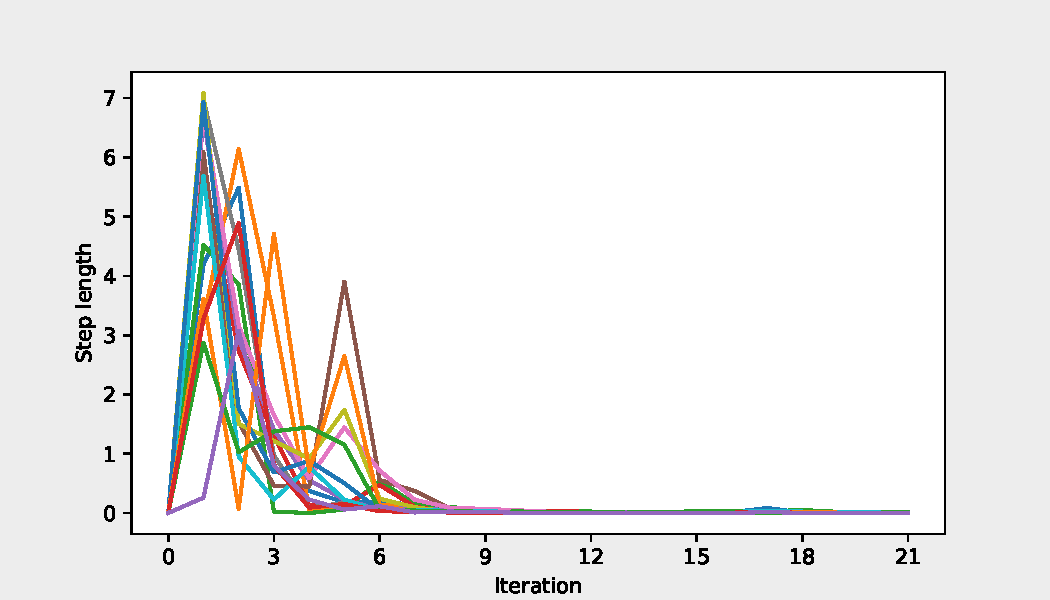
\includegraphics[width=\textwidth]{figs/bigworld_15_agnt_k_1_1_k_2_1_step_traj.pdf}
    \caption{Step length evolution for 15 agents in the Rectworld environment with $k_{1} = k_{1} = 1$ (active dispersion).}
    \label{fig:15_agnt_bw_k_1_1_s_traj}
  \end{subfigure}
  \caption{Coverage percentage and step length evolution for 15 agents in the Rectworld environment when active dispersion is used.}
  \label{fig:15_agnt_bw_evolution_active}
\end{figure}
\clearpage
\subsection{Complexworld}\label[secc]{complexworld}
The Complexworld is constructed to evaluate the performance of Algorithm \ref{alg:alg1} for a large swarm in a larger and more demanding environment.
Simulations are performed with and without active dispersion for a swarm of 50 agents. The results are shown in 
\Crefrange{fig:50_agnt_cw_k_1_0_k_2_1_distr}{fig:50_agnt_tw_evolution_active}.
\begin{figure}[H]
  \centering
  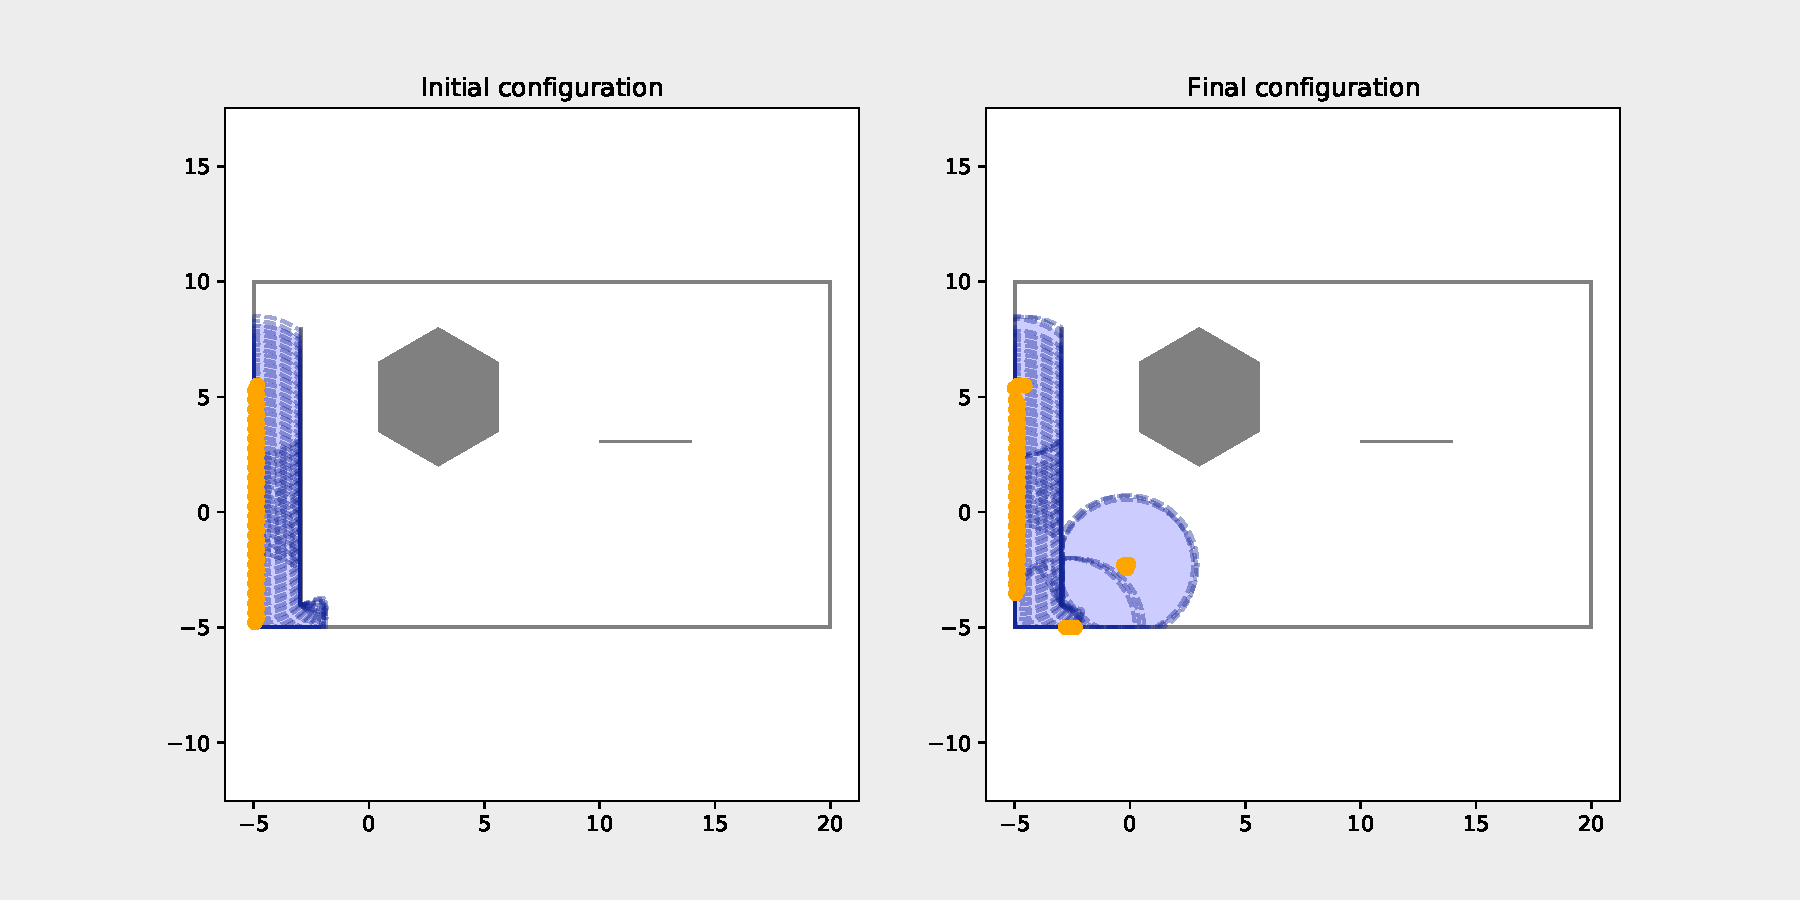
\includegraphics[width=\textwidth]{figs/complexworld_50_agnt_k_1_0_k_2_1_distr.pdf}
  \caption{Initial and final configuration of 50 agents in the Complexworld environment with $k_{1} = k_{2} = 1$ (active dispersion).}
  \label{fig:50_agnt_cw_k_1_0_k_2_1_distr}
\end{figure}

\begin{figure}[H]
  \centering
  \begin{subfigure}[t]{0.5\textwidth}
    \centering
    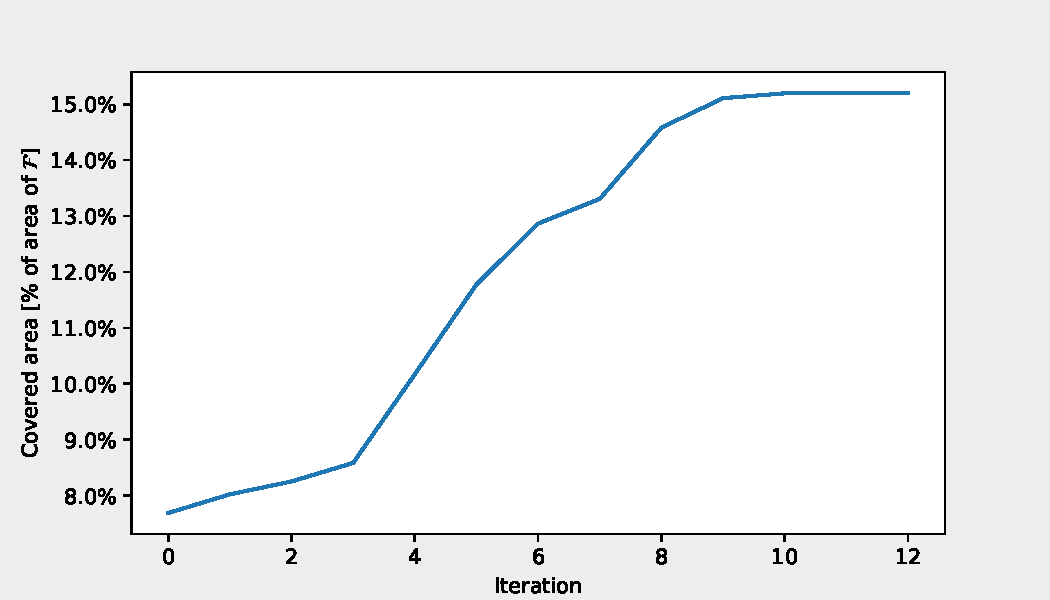
\includegraphics[width=\textwidth]{figs/complexworld_50_agnt_k_1_0_k_2_1_area_traj.pdf}
    \caption{Coverage evolution for 50 agents in the Complexworld environment with $k_{1} = k_{2} = 1$ (active dispersion).}
    \label{fig:50_agnt_cw_k_1_0_k_2_1_a_traj}
  \end{subfigure}%
  ~ 
  \begin{subfigure}[t]{0.5\textwidth}
    \centering
    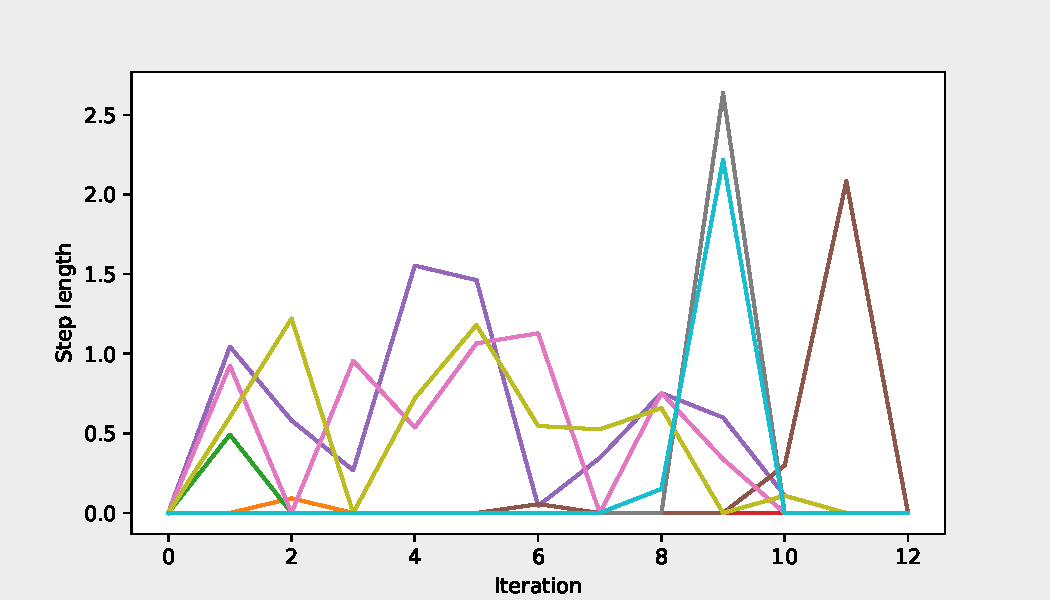
\includegraphics[width=\textwidth]{figs/complexworld_50_agnt_k_1_0_k_2_1_step_traj.pdf}
    \caption{Step length evolution for 50 agents in the Complexworld environment with $k_{1} = k_{2} = 1$ (active dispersion).}
    \label{fig:50_agnt_cw_k_1_0_k_2_1_s_traj}
  \end{subfigure}
  \caption{Coverage percentage and step length evolution for 50 agents in the Complexworld environment when active dispersion is used.}
  \label{fig:50_agnt_cw_evolution}
\end{figure}


\begin{figure}[H]
  \centering
  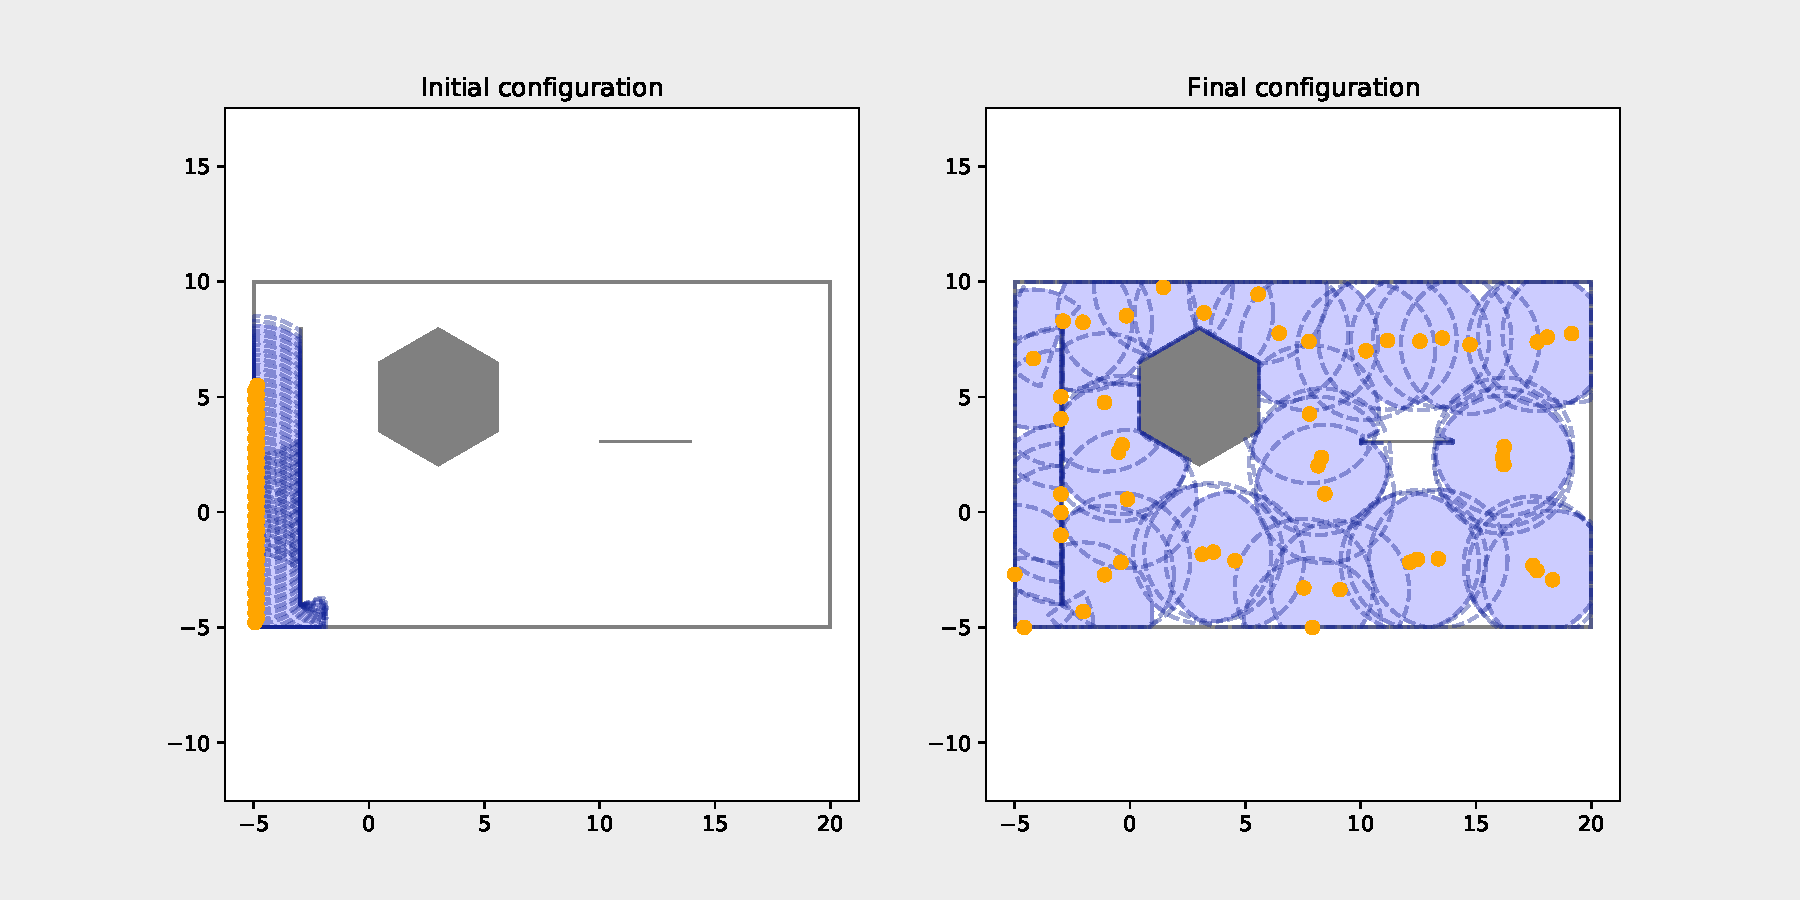
\includegraphics[width=\textwidth]{figs/complexworld_50_agnt_k_1_1_k_2_1_distr.pdf}
  \caption{Initial and final configuration of 50 agents in the Complexworld environment with $k_{1} = k_{2} = 1$ (active dispersion).}
  \label{fig:50_agnt_cw_k_1_1_k_2_1_distr}
\end{figure}

\begin{figure}[H]
  \centering
  \begin{subfigure}[t]{0.5\textwidth}
    \centering
    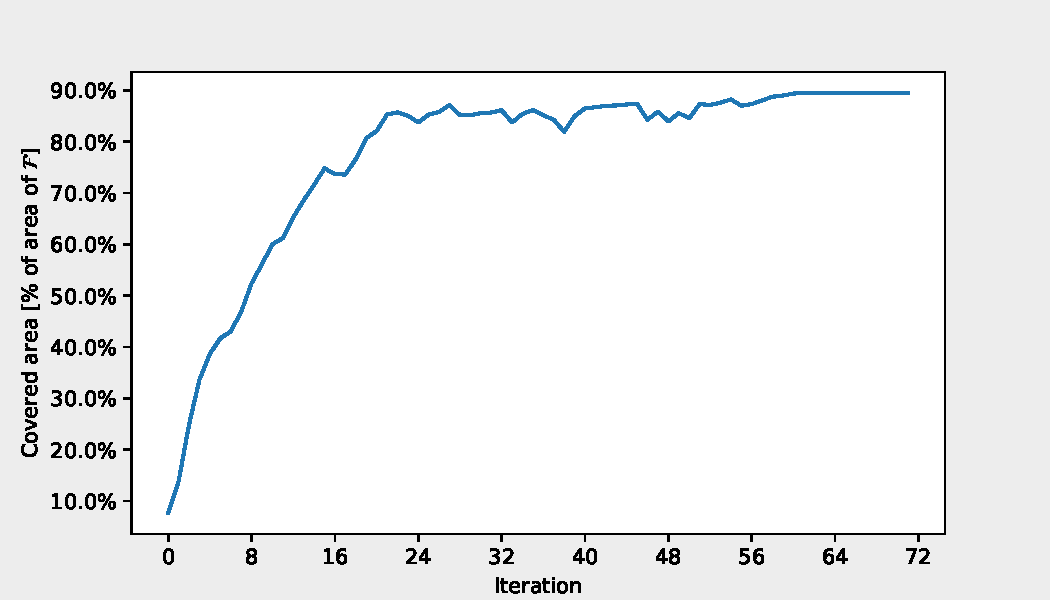
\includegraphics[width=\textwidth]{figs/complexworld_50_agnt_k_1_1_k_2_1_area_traj.pdf}
    \caption{Coverage evolution for 50 agents in the Complexworld environment with $k_{1} = k_{2} = 1$ (active dispersion).}
    \label{fig:50_agnt_cw_k_1_k_2_1_a_traj}
  \end{subfigure}%
  ~ 
  \begin{subfigure}[t]{0.5\textwidth}
    \centering
    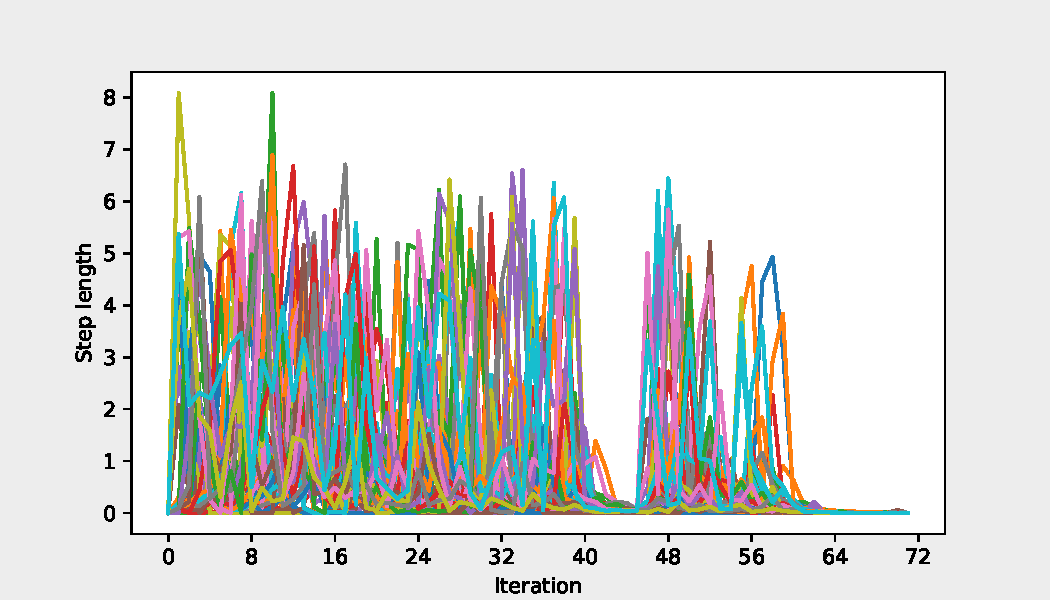
\includegraphics[width=\textwidth]{figs/complexworld_50_agnt_k_1_1_k_2_1_step_traj.pdf}
    \caption{Step length evolution for 50 agents in the Complexworld environment with $k_{1} = k_{2} = 1$ (active dispersion).}
    \label{fig:50_agnt_cw_k_1_1_k_2_1_s_traj}
  \end{subfigure}
  \caption{Coverage percentage and step length evolution for 50 agents in the Complexworld environment when active dispersion is used.}
  \label{fig:50_agnt_tw_evolution_active}
\end{figure}
